%Paqueting
\documentclass[11pt, letterpaper, spanish]{article}
\usepackage[spanish]{babel}
\usepackage[utf8]{inputenc}
\usepackage[letterpaper, margin=2cm]{geometry}
\usepackage{graphicx}
\usepackage[rightcaption]{sidecap}
\usepackage{float}
\usepackage{array}
\usepackage{amsmath, amsthm, amssymb}
\DeclareUnicodeCharacter{2212}{-}
\usepackage{wrapfig}
\usepackage{enumerate} 
\usepackage{xcolor}
\usepackage[hidelinks]{hyperref} 
\usepackage{latexsym}
\usepackage{hyperref}
\graphicspath{{images/}} 
\hypersetup{
    colorlinks=true,
    linkcolor=black,
    filecolor=blue,      
    urlcolor=blue,
    citecolor=black,
    pdftitle={Manual de modelado de proyectos para futuros equipos de iGEM},
    pdfpagemode=FullScreen,
    }
\usepackage{titlesec}


\setcounter{secnumdepth}{4}

\titleformat{\paragraph}
{\normalfont\normalsize\bfseries}{\theparagraph}{1em}{}
\titlespacing*{\paragraph}
{0pt}{3.25ex plus 1ex minus .2ex}{1.5ex plus .2ex}



%Dates
\title{Manual de modelado de proyectos para futuros equipos de iGEM}
\author{iGEM UAM \&  iGEM Tec-Chihuahua \& }

\begin{document}

\begin{titlepage}
   \begin{center}
       
   {\Huge \textbf{Manual de modelado de proyectos para futuros equipos iGEM}}

       \vspace{0.5cm}
        Una mirada al modelado matemático/informático en la biología sintética
            
       \vspace{1.5 cm}

\centering\begin{tabular}{>{\centering\arraybackslash} c c c}
iGEM UAM &  & iGEM Tec-Chihuahua \\
igem.uam@gmail.com &  & igemtecchihuahua@gmail.com\\
Universidad Autónoma Metropolitana &  & Instituto Tecnológico y de Estudios\\
 &  & Superiores de Monterrey, Campus Chihuahua\\
 &  & \\
 \end{tabular}
 \centering\begin{tabular}{>{\centering\arraybackslash} c}
 USP-EEL-Brazil \\
symb-lab@usp.br \\
Universidade de São Paulo \\
Escola de Engenharia de Lorena \\
\end{tabular}

  \vspace{1.0cm}
        

\includegraphics[width=12cm]{Logos-Chih-UAM-USP.png}

       \vfill
       \vspace{0.8cm}
       Brasil, México\\
       Julio 2022
            
   \end{center}
\end{titlepage}


\title{Manual Modelado Matemático}


\nocite{*}

\newpage

\tableofcontents

\newpage
\section{Introducción}
\par{La modelación matemática y computacional constituye uno de los pilares fundamentales de la ciencia contemporánea. Gracias a ella, los investigadores pueden predecir con éxito el comportamiento de muchos sistemas, desde el clima, los pozos de petróleo, las células y los acuíferos hasta la interacción de las galaxias. Hay múltiples formas de modelar la realidad. Podemos usar álgebra, geometría o muchas otras herramientas matemáticas. Sin embargo, la mayoría de ellos se hacen usando ecuaciones diferenciales \cite{castillo_2012}.}

\par{Las ecuaciones diferenciales son usadas porque capturan la naturaleza dinámica de nuestro mundo. Muestran cómo cambia algo dependiendo de otra cosa (por ejemplo, una cubeta que se mantiene bajo un grifo abierto se llena de agua después de cierto tiempo\footnote{En este caso mediremos la cantidad del agua en la cubeta (nuestra función variable) En dependencia del tiempo (nuestra función independiente)}). Cuando solo se mide el cambio de una variable, las ecuaciones se denominan ecuaciones diferenciales ordinarias (EDO).}

\par{Los modelos más completos miden cómo cambian las variables dependiendo no solo de una variable independiente (tiempo, por ejemplo) sino también de otras variables independientes (temperatura, presión, etc.).}

\par{Un modelo matemático no es foco de atención por su complejidad estructural o su magnífica formulación teórica. Puede limitarse a ser una aproximación aceptable de la realidad. Un modelo simple podría ser útil si incorpora conocimientos científicos, como las leyes generales de la naturaleza y conocimientos tecnológicos, como las mediciones experimentales. Todos los modelos útiles, ya sean explicativos o no, son predictivos: nos permiten hacer predicciones cuantitativas (ya sean deterministas o probabilísticas) que pueden usarse para probar y refinar el modelo, en caso de que sea necesario, o para su uso en la práctica.}

\par{El modelado matemático muestra la aplicabilidad de todo tipo de ideas matemáticas a problemas del "mundo real". Algunos de estos surgen en los intentos de explicar los fenómenos naturales, por ejemplo, los modelos de ondas de agua. Otras aplicaciones se encuentran en la industria, que es una fuente de muchos problemas matemáticos fascinantes y no estándar. Los procesos industriales no están definidos en detalle. Las condiciones críticas hacen que sea costoso y difícil realizar investigaciones experimentales detalladas. Aunque los ingenieros y otros profesionales diseñan procesos que funcionan bien y son eficientes. Entonces, ¿dónde entran las matemáticas? Algunos usos importantes son el control de calidad y el control de costes de los procesos existentes y la simulación y el diseño de otros nuevos. Es posible que queramos entender por qué ocurre cierto tipo de defecto; cuál es la parte de "limitación de la velocidad" de un proceso; cómo mejorar la eficiencia, aunque sea marginalmente; si es probable que una idea novedosa funcione y, de ser así, cómo controlarla \cite{Howison_2008}.}

\par{Este manual se basa en el trabajo del equipo iGEM de Imperial College London de 2020, en su guía: \href{https://static.igem.org/mediawiki/2020/9/96/T--Imperial_College--introtomodelling.pdf}{"Introducción al Modelado Matemático en Biología Sintética: Versión 1"}. Al igual que nuestros antecesores, extendemos la invitación a cualquier equipo de iGEM para traducir o mejorar nuestro trabajo con absoluta libertad. El archivo fuente LaTeX se puede encontrar en nuestra página wiki y \href{https://github.com/Rexmali/iGEM-UAM2022}{aquí}.}

\par{El objetivo de este manual es ampliar la excelente guía de \cite{igem_2020} con un enfoque práctico. Debido a este objetivo, queremos presentar las bases teóricas de la Modelación Matemática y su implementación computacional.}

\newpage 

\section{Justificación}
\par{Cuando comenzamos a desarrollar nuestros proyectos, estábamos muy emocionados de poder contribuir a nuestra comunidad a través de la biología sintética. Nos inspiramos del excelente trabajo que los equipos habían hecho en ediciones pasadas. Esto nos llevó a buscar que cada una de las áreas que desarrollamos en nuestros proyectos fueran sobresalientes. No obstante, al inicio de nuestro proyecto, uno de los primeros retos que enfrentamos fue iniciar el modelo, sentimos que no sabíamos por dónde empezar, hablando con otros equipos de iGEM nos dimos cuenta de que compartimos ese mismo pensamiento. Además, notamos que el área de modelado del proyecto representa un reto desde que muchos de los equipos de la competencia su primer enfoque es modelar sistemas biológicos. }
\par{En la mayoría de los cursos universitarios, incluso en los enfocados en biotecnología, las materias de bioinformática no son suficiente para enseñar las herramientas de modelado matemático necesarias para la competencia. Las clases de programación en ingeniería y los cursos de computación no enseñan sobre modelado de proteínas. Así que como la universidad no nos prepara para esto, necesitamos algo que nos prepare.}
\par{El modelado de un proyecto es una parte fundamental del diseño de cualquier trabajo. Este consiste en la descripción de un sistema complejo a través de fórmulas matemáticas, simulaciones computacionales y dinámicas moleculares entre otras. El modelado de un proyecto permite predecir el comportamiento de un sistema antes de su construcción y los problemas pueden ser identificados, y evitar un gasto innecesario de tiempo y dinero.}
\par{Por supuesto, la autonomía del estudiante es importante en el proceso de aprendizaje, pero la idea de “aprender aprendiendo” que sucede en el modelo es algo anticuado. Muchos equipos han dejado un increíble legado en el área de bioinformática, pero hay una falta de contenido para ayudarlos a aprender, y este proceso puede ser agotador. Si el modelado es una herramienta, como se dice, ayuda a ahorrar tiempo en el laboratorio, ¿por qué no ahorrar tiempo al desarrollarlo? Ciertamente, una persona responsable por el modelo tendrá que usar sus pensamientos para interpretar sus resultados y construir sistemas, pero no hay suficiente información sobre cómo usar el software o cómo elegir el mejor según nuestras necesidades.}
\par{Fueron meses de investigación, asesoramiento, autoaprendizaje y apoyo entre equipos para desarrollar buenos modelos. Durante el desarrollo de la competencia aprendimos muchísimo. Sin embargo, estamos conscientes que, si el conocimiento no se comparte, es inútil. Así que decidimos una manera en la que el conocimiento que hemos adquirido trascienda y es así como nació la idea del manual.}
\par{Asimismo, vimos el manual como una forma de devolver todo el apoyo que hemos recibido para el desarrollo de nuestros proyectos. A lo largo de nuestra historia en iGEM, hemos recibido ayuda de muchas personas como mentores, instructores y otros equipos que nos han apoyado en nuestro proyecto, especialmente en modelado. Sin ellos, el desarrollo de nuestros proyectos no habría sido posible. Así como ellos compartieron su conocimiento y su experiencia con nosotros, queremos compartir con otros equipos de iGEM alrededor del mundo, pero, principalmente, con equipos de Latinoamérica, es por eso que está disponible en inglés, español y portugués. Adicionalmente, es una manera de contribuir al desarrollo del conocimiento científico en nuestra lengua materna y de la misma manera, puede ser útil para la gente fuera de iGEM. Sin embargo, cada equipo de iGEM puede traducir este manual, así que cualquiera puede acceder a esta información.}
\par{Estamos conscientes que la diversidad nos enriquece y nos ayuda a ir más allá. Es por eso que nosotros como equipos no angloparlantes, iGEM Tec Chihuahua, iGEM UAM de México y USP-EEL de Brasil nos unimos para trabajar en este manual.  Entendemos la necesidad de otros equipos de iGEM de obtener conocimiento científico en nuestra respectiva lengua materna. Al ser parte de los pocos equipos de LATAM que participarán este año en la competencia nos hace querer contribuir con algo valioso para la comunidad de iGEM.
No menos importante, estamos agradecido con el equipo del Imperial College London por permitir basarnos en su manual hecho en 2020.
Por lo que, sumando el conocimiento de cada equipo y el conocimiento que hemos desarrollado juntos trabajando hombro a hombro, buscamos generar diferentes perspectivas sobre el proyecto de modelado.}
\par{Esperamos que este manual sirva como una primer guía para futuros equipos.}



\section{Objetivos}

\begin{enumerate}
    \item Describir, explicar y facilitar los principios de un modelo matemático a los equipos iGEM de Latinoamérica.
    \item Explicar los tipos de modelos matemáticos que pueden utilizarse y las ventajas que presentan modelando diferentes fenómenos biológicos.   
    \item Describir las herramientas bioinformáticas disponibles para implementar en un proyecto iGEM.
    \item Comprender cómo es posible realizar simulaciones computacionales de los modelos matemáticos con un enfoque biológico.
    \item Ejemplificar modelos de sistemas biológicos que puedan servir de base para nuevos trabajos.
    
\end{enumerate}
\newpage

\newpage
\section{Herramientas matemáticas}
\subsection{Ecuaciones Diferenciales}
\par{Una ecuación diferencial (ED) es una relación entre una función del tiempo y sus derivadas. Las ecuaciones diferenciales pueden presentarse de muchas formas y son un concepto esencial para las matemáticas y la ciencia. Las ecuaciones \ref{eq1} y \ref{eq2} son ambas ejemplos de ecuaciones diferenciales. Al modelar la dinámica de un sistema donde las variables varían con el tiempo, podemos formar ED para modelar esta variación. Los procesos celulares, como la transcripción y la traducción, toman tiempo, por lo que debemos describir la variación de las concentraciones de ARNm y proteína mediante ecuaciones diferenciales y luego intentar resolver esas ecuaciones. }

\begin{equation}
    \frac{d y}{d t}=3 y^2 \sin{\left( x+t  \right)}
    \label{eq1}
\end{equation}

\begin{equation}
    \frac{d^3 y}{{d t}^3}=\exp{-y} + t + \frac{d^2 y}{{d t}^2}
    \label{eq2}
\end{equation}

\subsubsection{Caracterización}

\par{Las propiedades de las ecuaciones diferenciales y sus soluciones se pueden analizar a partir de su caracterización. El contar con una comprensión básica de estas categorías es útil.}

    \paragraph{ El orden de una ecuación diferencial}
    
    \par{El orden de una ecuación diferencial es el orden de la mayor derivada de la función que aparece en la ecuación. Por lo tanto, la Ecuación \ref{eq1} es una ecuación diferencial de primer orden y la Ecuación \ref{eq2} es una ecuación diferencial de tercer orden.}

    \paragraph{ Número de variables independientes}
    
    \par{\textit{Las ecuaciones diferenciales ordinarias} (EDO) tienen una variable dependiente (y sus derivadas) que solo depende de una variable independiente.\textit{ Las ecuaciones diferenciales parciales} (EDP), por otro lado, tienen una variable dependiente que depende de dos o más variables independientes. Las PDE son mucho más complejas de resolver. }
    
    \paragraph{Homogeneidad de la ecuación diferencial}
    
    \par{La Ecuación \ref{eqhomo} se denomina ecuación diferencial lineal homogénea de primer orden, y la Ecuación \ref{eqhomo2} se denomina ecuación diferencial lineal de primer orden no homogénea para b(t) no idénticamente cero. Homogéneo significa que cada término contiene la variable dependiente o sus derivados, mientras que no homogéneo implica que hay al menos un término que no la contiene.}

     \begin{equation}
        \frac{d y}{d t}+a(t) y =0
        \label{eqhomo}
    \end{equation}
    
    \begin{equation}
        \frac{d y}{d t}+a(t) y =b(t)
        \label{eqhomo2}
    \end{equation}

    
    \paragraph{ Linealidad de la ecuación diferencial}
     \par{Lineal implica que cada término tiene la forma coeficiente × derivada, de modo que la variable dependiente y sus derivadas nunca están en la función. Llamamos ecuación lineal porque la variable dependiente y aparece sola, es decir, sin términos como $e^{-y}$, $y^3$ o $\sin{(y)}$ etc. aparecen en la ecuación. Por ejemplo, $\frac{dy}{dt} = y^2 + \sin{t}$ y $\frac{dy}{dt} = \cos{(y)} + t$ ambas son ecuaciones no lineales debido a los términos $y^2$ y $\cos{(y)}$ respectivamente \cite{braun_1993}. 

     \paragraph{ Sistemas de ecuaciones diferenciales }
    
    \par{Cuando se encuentra acoplado, esto implica que hay dos o más ED en las que se comparten dos o más variables dependientes. De esta forma, la variación de la variable dependiente de una ED depende de la variación de la variable dependiente de otra ED. Los sistemas de ED tienen la forma: }

    \begin{equation}
    \begin{split}
    \frac{d x_1}{dt}=f_1(t,x_1,x_2,...,x_n)\\
    \frac{d x_2}{dt}=f_2(t,x_1,x_2,...,x_n)\\
    . \\
    . \\
    . \\ 
    \frac{d x_n}{dt}=f_n(t,x_1,x_2,...,x_n)
    \end{split}
    \end{equation}

    \subsubsection{Soluciones}
     \par{Las soluciones de una ED son funciones que satisfacen la ecuación tal que no hay derivadas en la solución. Muchas veces, las ED no se pueden resolver analíticamente (es decir, una solución algebraica general). Esto se debe a que la integración a veces es imposible para ecuaciones más complejas (como la ecuación de Hill, en general). Sin embargo, pueden resolverse numéricamente usando métodos computacionales iterativos. Hay muchos métodos diferentes para diferentes situaciones, pero programas como MATLAB o paquetes como Scipy en Python tienen funciones que hacen el trabajo duro.}

      \subsection{Cinética de acción de masas (CAM)}
    
    \par{La cinética de acción de masas es un marco para analizar reacciones químicas basado en la suposición de que la velocidad de las reacciones se puede modelar mediante la concentración de los reactivos. También hay un coeficiente de proporcionalidad que se encuentra empíricamente. Una vez que se conocen estos coeficientes, la ecuación de velocidad (a DE) se puede resolver para proporcionar un modelo que describa cómo varían las concentraciones con el tiempo.}
     \par{Las siguientes secciones describen diferentes casos en los que se utiliza esta ley.}
      \subsubsection{Una reacción simple}

    \par{Considere la siguiente reacción}

    \begin{equation}
        A \rightarrow C.
    \end{equation}

    \par{Por cada A que reacciona, se genera un C como producto. Es decir, por cada reacción, se crea una C y se agota una A. Dado que C no reacciona, las tasas no dependerán de C. En esta ecuación, modelaríamos las tasas como se muestra en la Ecuación \ref{Eq7} y la Ecuación \ref{Eq8}. }

    \begin{equation}
        \frac{d [A]}{d t}=-k[A]
        \label{Eq7}
    \end{equation}

    \begin{equation}
        \frac{d [C]}{d t}=k[A]
        \label{Eq8}
    \end{equation}

    \par{Donde k es una constante que describe la velocidad relativa de la reacción. A medida que se consume A, la concentración disminuye. A medida que se produce C, la concentración aumenta. Dado que la tasa de producción de C es equivalente a la tasa de uso de A, las ecuaciones son muy similares.}

    \subsubsection{Reacción inversa}

    \par{Supongamos que introducimos la reacción inversa, para que C pueda reaccionar y volver a A: }

    \begin{equation}
        A \rightleftharpoons C.
    \end{equation}

     \par{Esto significaría que efectivamente tenemos dos reacciones, A a C y C a A. Las nuevas velocidades son la suma de estas dos EDO. Por lo tanto, en total, tenemos las siguientes ecuaciones [\ref{Eq10}, \ref{Eq11}]. }

     \begin{equation}
        \frac{d [A]}{d t}=-k_1[A]+k_2[C]
         \label{Eq10}
    \end{equation}


    \begin{equation}
        \frac{d [C]}{d t}=k_1[A]-k_2[C]
         \label{Eq11}
    \end{equation}

 \subsubsection{Dos reactivos}

    \par{Aumentemos la complejidad y agreguemos un reactivo adicional:}
    \begin{equation}
        A+B \rightleftharpoons C.
        \label{eq12}
    \end{equation}

\par{Intuitivamente, vemos que un A y un B deben reaccionar para formar un C. Esto significa que si no hay A, no ocurrirá la reacción. Implica que la tasa depende de la concentración de A y B en una combinación de término. Del mismo modo, la reacción inversa solo depende de C y produce un A y un B. Por lo tanto, tenemos 3 tasas: }

\begin{equation}
        \frac{d [A]}{d t}=-k_1[A][B]+k_2[C]
        \label{eq13}
    \end{equation}

    \begin{equation}
        \frac{d [B]}{d t}=-k_1[A][B]+k_2[C]
        \label{eq14}
    \end{equation}

    \begin{equation}
        \frac{d [C]}{d t}=k_1[A][B]-k_2[C]
    \end{equation}

    \par{Tenga en cuenta que la velocidad de cambio de A y B es igual porque la reacción ocurrirá sin ningún reactivo.}

    \subsubsection{Coeficientes de reacción}

    \par{Considere la reacción}

    \begin{equation}
        2A \rightleftharpoons C.
        \label{eq16}
    \end{equation}

    \par{Haciendo referencia a la sección C, observamos que las tasas estarán dadas como se muestra en la Ecuación \ref{eq17} y en la Ecuación \ref{eq17}. }

     \begin{equation}
        \frac{d [A]}{d t}=-k_1[A][A]+k_2[C]=-k_1{[A]}^2+k_2[C]
        \label{eq17}
    \end{equation}

    \begin{equation}
        \frac{d [C]}{d t}=k_1[A]^2-k_2[C]
        \label{eq18}
    \end{equation}

    \par{Entonces, el coeficiente en la ecuación de reacción será la potencia en la ecuación de velocidad. Y podemos generalizar las Ecuaciones  (\ref{eq12}), (\ref{eq13}) y (\ref{eq16}), como: }

    \begin{equation}
        nA+mB \rightleftharpoons C.
    \end{equation}

    \par{Con el cambio de tasa:}

    \begin{equation}
        \frac{d [A]}{d t}=\frac{d [B]}{d t}=-k_1{[A]}^n[B]^m+k_2[C]
    \end{equation}

    \par{y}

    \begin{equation}
        \frac{d [C]}{d t}=k_1[A]^n[B]^m-k_2[C]
    \end{equation}
   
    \subsubsection{Degradación}

    \par{En algunos casos, una molécula puede degradarse a alguna otra especie que no es relevante para el sistema en sí, y no puede volver a la molécula original. Escribimos esto como:}
    \begin{equation}
        A \longrightarrow  \varnothing
    \end{equation}
    \par{Esto se modela igual que en la parte A, pero no hay producto. En cambio, lo ignoramos, ya que solo nos importan ciertas especies dentro de un sistema. El coeficiente de tasa de degradación se suele dar como $\delta$, se puede observar en la ecuación [\ref{eq23}].}

 
    \begin{equation}
        \frac{d [A]}{d t}=-\delta[A]
        \label{eq23}
    \end{equation}

    \par{Esto se modela igual que en la parte A, pero no hay producto. En cambio, lo ignoramos, ya que solo nos importan ciertas especies dentro de un sistema. El coeficiente de tasa de degradación se suele dar como as $\delta$, dada su tasa de la ecuación.}

    \subsubsection{Ejemplo}
    
    \par{Dada la ecuación química para la producción de cloruro de hidrógeno a partir de hidrógeno y cloruro, encuentre la ecuación de velocidad correcta para el cloruro de hidrógeno (la velocidad de reacción directa es igual a $K_F$ y la inversa de la velocidad de reacción es de $K_B$):}
    \begin{equation}
        H_2+{Cl}_2 \rightleftharpoons 2HCl
    \end{equation}
    
    \vspace{2 cm}
    
    \begin{equation}
        A)\frac{d [HCl]}{d t}=+k_F[H_2][{Cl}_2]-k_B[HCl]^2
    \end{equation}

    \begin{equation}
        B)\frac{d [HCl]}{d t}=+k_F[H_2][{Cl}_2]-k_B[HCl]
    \end{equation}

    \begin{equation}
        C)\frac{d [HCl]}{d t}=+k_F{[H]}^2{[Cl]}^2-k_B[HCl]^2
    \end{equation}

    \subsection{ Ecuación de Hill}
    \par{En cualquier reacción en la que dos especies se unen, pueden separarse y volver a sus partes constituyentes. Esta es la misma forma que en la sección 2.2.3, pero donde las especies más grandes pueden tener múltiples sitios de unión, por lo que tenemos una ecuación de reacción de la siguiente forma:}
    
    \begin{equation}
    A+mB \rightleftharpoons C.
    \end{equation}

    \par{Donde A es la especie más grande, B es la especie más pequeña, C es el complejo formado por la unión y n es el número de sitios de unión en A. Por ejemplo, la unión de un ligando a una macromolécula, un factor de transcripción a un promotor, o un sustrato para una enzima. Usando CAM, podemos derivar una ecuación llamada Ecuación de Hill, a partir de la ecuación de la tasa, en base a algunas suposiciones. Si bien tiene limitaciones en cuanto a su precisión, la ecuación de Hill es un buen punto de partida cuando se desconoce la dinámica de la unión.}

    \subsubsection{Derivación}
    
    \par{Definimos la constante de reacción directa $k_a$ para la asociación y la constante de reacción inversa $k_d$ para la disociación.}

    \begin{equation}
        \frac{d [C]}{d t}=k_A{[A]}[B]^m+k_d[C]
    \end{equation}

    \par{Si $[C]$ es inicialmente cero, las concentraciones cambiarán hasta que la velocidad de reacción directa sea igual a la velocidad de reacción inversa, de modo que las concentraciones ya no varíen con el tiempo. A este punto lo llamamos equilibrio. Esto significa que, en equilibrio, la concentración del complejo no variará con el tiempo. Por lo tanto, igualamos esta ecuación a cero:}

    \begin{equation}
        \frac{d [C]}{d t}=k_A{[A]}[B]^m+k_d[C]=0
    \end{equation}

    \par{Reordenando, definimos la constante de disociación aparente, $K_d$, como la relación de la tasa de disociación constante y la tasa de asociación constante.} 

    \begin{equation}
        K_d = \frac{k_d}{k_a}=\frac{[A]{[B]}^m}{[C]}
        \label{eq31}
    \end{equation}

    \par{ Entonces podemos calcular la proporción de moléculas A unidas a la proporción de moléculas A totales (unidas y no unidas), que llamamos $\theta$: }

    \begin{equation}
        \theta= \frac{Bound A molecules}{Total A molecules}=\frac{[C]}{[A]+[C]}
    \end{equation}
    
    \par{Recordando que A es la especie más grande.}
    
    \par{Usando la ecuación (\ref{eq31}), podemos sustituir [C] = [A][B]n Kd y reorganizar para obtener la ecuación.} 
    
    \par{Esta es la proporción de la molécula compleja (A unida) al número total de moléculas A en términos de su concentraciones. También es posible encontrar la proporción de moléculas A no unidas, simplemente calculando $(1-\theta)$}.

    \begin{equation}
        \theta = \frac{ \frac{[A]{[B]}^m}{K_d} }{ [A] + \frac{[A]{[B]}^m}{K_d} }= \frac{[A]{[B]}^m}{[A] K_d + [A] {[B]}^m} = \frac{{[B]}^m}{ K_d + {[B]}^m}
    \end{equation}

    \subsubsection{Limitaciones}
    
    \paragraph{Asunciones}
    \par{Asume que todos los B se unen a A simultáneamente, a diferencia de en sucesión durante algún tiempo.}
     \par{No toma en cuenta la interacción entre los B sucesivos y su cooperatividad (este modelo asume una cooperatividad muy positiva).}
 \par{ No considera la unión parcial (es decir, no se llenan todos los sitios de unión) y la funcionalidad de este complejo parcialmente unido.}

    

 \newpage  

\section{Modelos a utilizar y sus características}
\par{Un modelo matemático es una expresión formal (en lenguaje matemático) de las relaciones entre los componentes de un modelo. Construir un modelo de este tipo implica seleccionar y cuantificar los componentes variables y relaciones presentes en el sistema para representarlo con el nivel de detalle requerido. Puede ser algo tan simple como sustituir las variables de una ecuación por sus valores reales o puede ser un conjunto complejo de ecuaciones interrelacionadas cuyas variables se modifican a lo largo del tiempo y a través del espacio.}
\par{El lenguaje matemático permite describir y modelar sistemas de forma parsimoniosa, objetiva e inequívoca; hasta el punto de que hoy en día los modelos matemáticos son considerados como representaciones de teorías sobre los sistemas que se están modelando. El lenguaje simbólico proporcionado por las matemáticas permite la expresión de ideas altamente complejas.}
Se debe hacer una distinción entre esta concepción de un modelo, como una representación de una teoría por medio de una ecuación más o menos simple, y la idea de un modelo como un grupo de un conjunto de ecuaciones (que responden a diferentes teorías) interconectadas de una manera que representa las diferentes transferencias entre los componentes del sistema modelado. 
\par{Las características deseables de los modelos matemáticos son:}

\subsection{Características}
\begin{itemize}
    \item Parsimonia, un modelo no es necesariamente mejor por tener muchos parámetros. la simplicidad siempre es deseable.
    \item Modestia, deben tratar de lograr solo objetivos alcanzables. Un modelo, como un mapa, no debe aspirar a imitar la realidad sino sólo a resaltar aquellos aspectos de interés para su aplicación.
    \item Precisión, el modelo debe reproducir en la medida de lo posible el funcionamiento del sistema y generar valores para las variables de salida y estado similares a los observados en la realidad.
    \item Verificabilidad, los resultados del modelo deben poder compararse con datos reales y determinar a partir de este modo el grado de precisión del modelo.
    \item Por otro lado, no basta con que funcionen bien, deben funcionar bien por las razones correctas.
    \end{itemize}.
    \begin{enumerate}
        \item Determinismo
    \par{Decir que un sistema es determinista significa que cada estado está completamente determinado por el estado anterior. 
    Por ejemplo, en el modelo de cadena alimentaria, al igual que en todos los demás modelos que hemos estudiado, no hay influencias externas no modeladas o eventos fortuitos. Si permitimos eventos fortuitos externos, es fácil producir una serie temporal irregular, por ejemplo, lanzando una moneda, pero no hay nada como esto en el modelo de cadena alimentaria o el modelo logístico discreto. El sistema está produciendo determinísticamente su propio comportamiento irregular sin ninguna aleatoriedad. \cite{garfinkel_shevtsov_guo_2017}.}
    \item{Acotamiento}
    \par{Significa que el sistema hasta el infinito, más bien, como ilustra la figura a continuación, permanece dentro de una cierta región del espacio. En otras palabras, podríamos dibujar una caja en un espacio estacionario y el sistema se quedaría dentro de esa caja. En el modelo logístico discreto, siempre y cuando nuestra condición inicial esté dentro del intervalo (0, 1), el resultado siempre estará en ese intervalo; el punto de estado no se irá a valores más altos \cite{garfinkel_shevtsov_guo_2017}.}
    
    \begin{figure}[ht]
	    \centering
		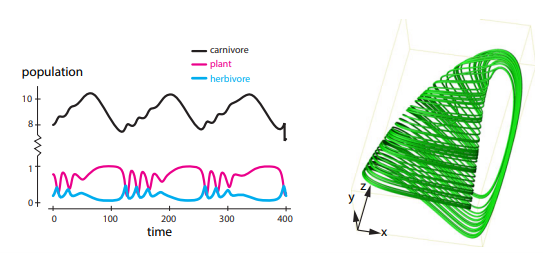
\includegraphics[width=0.7 \textwidth]{Chaos.png}
  \label{Imagen_1}
		\caption{Izquierda: una simulación del modelo de cadena alimentaria de tres especies descrito en el texto con a1 = 5, b1 = 3, a2 = 0.1, b2 = 2, d1 = 0.4 y d2 = 0.01. Derecha: una trayectoria típica del modelo de tres especies, Obtenido de: \cite{garfinkel_shevtsov_guo_2017}}
	\end{figure}
	\item{Irregularidad}
	\par{El comportamiento caótico es irregular o aperiódico. El comportamiento aperiódico nunca se repite exactamente. Si una trayectoria alguna vez se repitiera exactamente, es decir, volviera al mismo punto de estado matemático, tendría que ser periódica, porque el determinismo requeriría que volviera una y otra vez. Todas las órbitas cerradas son trayectorias periódicas, por lo tanto, los atractores de ciclo límite son órbitas periódicas cerradas. Los sistemas con atractores de ciclo puntual o límite tienen transitorios iniciales, pero luego se establecen en un comportamiento repetitivo. El comportamiento caótico, por otro lado, comienza irregular y permanece irregular. En algunos sistemas, puede parecer que el comportamiento se repite y puede acercarse mucho a los valores de estado anteriores, pero nunca repetirse exactamente \cite{garfinkel_shevtsov_guo_2017}.}
	 \begin{figure}[ht]
	    \centrado
		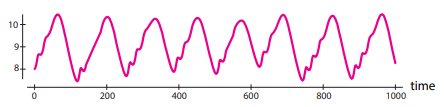
\includegraphics[width=0.7 \textwidth]{Irregularity.png}
		\label{Imagen_2}
		\caption{Serie temporal de la población de carnívoros a partir de una simulación típica del modelo de cadena alimentaria de las tres especies., (Obtenido de: \cite{garfinkel_shevtsov_guo_2017})}
	\end{figure}

 
    A primera vista, parece que las poblaciones oscilan, aunque de una manera algo compleja. Sin embargo, una mirada más cercana revela diferencias. La segunda gran oscilación contiene una protuberancia antes del pico, mientras que la tercera oscilación tiene al menos dos. Además, cada pico tiene una forma algo diferente. Esto es aperiodicidad. A pesar de una similitud cualitativa general, el comportamiento del sistema nunca se repite y nunca se acerca a la repetición. Una afirmación similar es cierta acerca de la salida del modelo logístico de tiempo discreto. Puede parecer que algunas formas se repiten, pero si miramos de cerca, vemos que la secuencia, de hecho, nunca se repite. \cite{garfinkel_shevtsov_guo_2017}
    
    \item{Dependencia sensible a las condiciones iniciales}
    \par{La característica más intrigante y famosa del caos es la dependencia sensible de las condiciones iniciales. Este término se refiere al hecho de que, en un sistema caótico, dos series temporales que comienzan muy juntas eventualmente divergirán hasta el punto en que su comportamiento no esté completamente correlacionado. En general, para sistemas multivariables, tanto en tiempo discreto como continuo, la dependencia sensible significa divergencia exponencial de trayectorias cercanas: hay un número $\lambda$ (letra griega lambda), llamado exponente característico de Lyapunov, tal que:} 
    
    \begin{equation*}
    d ( M_{t} − N_{t} ) = e^{ \lambda t} d ( M_{0} − N_{0} )  
    \end{equation*}

    \vspace{0,5 cm}

    \item{Imprevisibilidad}
    
    Quizás ya hayas oído hablar de Edward Lorenz, el meteorólogo y matemático que ayudó a descubrir el caos. Dio una reunión llamada "Previsibilidad: ¿el aleteo de las alas de una mariposa en Brasil desencadena un tornado en Texas?" Planteó una pregunta: Considere dos planetas que son absolutamente idénticos, hasta la ropa que usa hoy, cada árbol, cada detalle, excepto que en el mundo A hay una mariposa más en Brasil. ¿Qué pasará con los sistemas meteorológicos de los dos planetas? Tal vez pensaste que no habría diferencia con un cambio tan infinitesimal, pero el sentido común está equivocado. De hecho, después de no mucho tiempo, los sistemas meteorológicos divergirán por completo, de modo que hay, por ejemplo, un tornado en Texas en el mundo A, pero no en el mundo B. 
    La dependencia sensible de las condiciones iniciales ayuda a explicar una propiedad fundamental del comportamiento caótico, su imprevisibilidad. \cite{garfinkel_shevtsov_guo_2017}
    \end{enumerate}



\subsection{Modelos a usar}
\subsubsection{Derermínistico}
\par{El modelo determinista es un prototipo matemático, donde las mismas entradas producirán invariablemente las mismas salidas, independientemente de la consideración de la existencia de azar o incertidumbre. Conociendo con certeza los valores de las variables, entonces, se asumirá que tenemos toda la información necesaria para la evaluación de un proyecto\cite{ramos_2019}.}
\subsubsection{Estocásticos}
\par{Los modelos estocásticos se utilizan para representar la aleatoriedad y para proporcionar estimaciones de los parámetros de los medios que determinan el flujo de fluidos, el transporte de contaminantes y la transferencia de calor-masa en medios porosos naturales. Este modelo fue desarrollado por Ball en 1986, quien discutió que en la distribución de un período infeccioso se permite tener cualquier tipo de distribución que pueda ser descrita por su transformada de Laplace. Los modelos estocásticos se construyen alrededor de gráficos aleatorios. El proceso estocástico es el estudio de cómo evoluciona una variable aleatoria con el tiempo. Una variable que no se conoce antes de un cierto tiempo t se denomina variable aleatoria. Si el estado de la variable aleatoria se conoce antes de un tiempo finito, se denomina proceso estocástico discreto. El proceso de cadena de Markov es el mejor ejemplo de un modelo estocástico donde la distribución de probabilidad del tiempo t + 1 depende del estado en el tiempo t y no depende de los estados antes del tiempo t \cite{statistical_models_2003}.}
\subsubsection{Método Monte Carlo}
\par{Es una técnica matemática utilizada para estimar los posibles resultados de un evento incierto. El método Monte Carlo fue inventado por John von Neumann y Stanislaw Ulam durante la Segunda Guerra Mundial para mejorar la toma de decisiones en condiciones de incertidumbre. Su nombre proviene de un conocido casino en Mónaco, ya que el elemento de azar está en el centro del enfoque de modelado, similar a un juego de ruleta. Las simulaciones de Monte Carlo han evaluado el impacto del riesgo en muchos escenarios de la vida real, incluida la inteligencia artificial, los precios de las acciones, la previsión de ventas, la gestión de proyectos y los precios. También proporcionan una serie de beneficios para los modelos predictivos con entradas fijas, como la capacidad de realizar análisis de sensibilidad o calcular la correlación de entrada. El análisis de sensibilidad permite a los responsables de la toma de decisiones ver el impacto de las entradas individuales en un resultado dado, y la correlación les permite comprender las relaciones entre las variables de entrada\cite{garfinkel_shevtsov_guo_2017}.}
\subsubsection{Optimización}
\par{Se han hecho muchos esfuerzos para describir situaciones humanas y sociales complejas. Esto debe escribirse en una expresión matemática que contenga una o más variables, sus valores deben estar determinadas. La pregunta que se formula, en términos generales, es para qué valores estas variables deben tener una expresión matemática que tenga el mayor valor numérico posible (maximización) o el menor valor numérico posible (minimización). Este proceso general de maximización o minimización se denomina optimización. La optimización, se utiliza para encontrar la respuesta que proporciona el mejor resultado, la que logra los mayores beneficios, producción o felicidad, o la que logra el menor costo, desperdicio o incomodidad. Con frecuencia, estos problemas implican el uso más eficiente de los recursos, como dinero, tiempo, maquinaria, personal, inventario, etc. Los problemas de optimización generalmente se clasifican como lineales y no lineales, dependiendo de si las relaciones del problema con respecto a las variables.\cite{Arsham_1996}}
\subsubsection{Complejos}
\par{Un modelo complejo constituye la descripción matemática de un objeto complejo, el que consiste en elementos componentes interrelacionados, que también pueden estar constituidos por sus propios elementos interrelacionados. Además, el objeto complejo y sus elementos tienen funciones que también se pueden descomponer en el tiempo, porque en el caso general se requiere tomar decisiones relacionadas con el sistema en diferentes períodos. Sobre el sistema y sus elementos actúan interferencias del mundo circundante. Mientras más completa sea la organización del sistema más pequeña serán las interferencias, pero mayor la complejidad de la conciliación de la operación \cite{garfinkel_shevtsov_guo_2017}.}
    \par{La diferencia entre las palabras complejo y complicado son las siguientes:
    \begin{itemize}
        \item Complicado es algo que consta de muchas partes o detalles diferentes y, por lo tanto, difícil de entender, pero puede resolver un problema complicado analizando por separado las diferentes partes.
        \item Complex derivado del latín cum (muchos) plexus (participio pasado "complecti" que significa apretar, abrazar. Por lo tanto, una situación compleja, un sistema o problema complejo resultante de la unión de varias partes o elementos, se vuelve inseparable.
    \end{itemize}}

\subsubsection{Caóticos}
    \par{El concepto de caos es uno de los mayores descubrimientos de los últimos tiempos. El caos se observa en la vida cotidiana, en las áreas de metrología, flujo de fluidos (turbulencia), cardiología, biología de poblaciones, mercado de valores, modelización económica, etc. Las predicciones son posibles en muchos sistemas. Por ejemplo, los eclipses se pueden predecir con miles de años de anticipación. El movimiento de un péndulo simple (bajo supuestos adecuados), que se rige por una ecuación diferencial, es predecible y se puede escribir una solución de forma cerrada. Sin embargo, hay muchos fenómenos naturales que no son predecibles, como las predicciones meteorológicas, tirar los dados, etc., a pesar de que obedecen a las mismas leyes de la física. Se cree hasta hace poco que la previsibilidad se puede lograr teniendo más información y procesándola. Algunos sistemas son caóticos, extremadamente sensibles a pequeñas perturbaciones e impredecibles a largo plazo, mostrando el llamado efecto mariposa \cite{garfinkel_shevtsov_guo_2017}.}

    
    

\newpage

\section{Herramientas computacionales en modelado}

\par{Para la construcción de un modelo matemático el primer paso es plantear la estructura que queremos que tengan las ecuaciones diferenciales que usaremos y posteriormente transformar esas ecuaciones diferenciales parciales en un sistema que tenga un número finito de grados de libertad, esto significa que el sistema dependa de un número finito de variables y parámetros: podemos tener sistemas de tres, diez o mil variables. Algunas de esas ecuaciones requieren millones de variables.}

\par{Una ecuación sencilla tiene una sola incógnita, un sistema de tres variables generalmente tiene 3 incógnitas. Pero cuando se trata de modelar sistemas de la realidad se requiere transformar las ecuaciones diferenciales en sistemas de ecuaciones que involucran un número muy grande de incógnitas, pueden ser millones. Para pasar de una ecuación diferencial parcial a un sistema con un número finito de grados de libertad se hace por medio de métodos numéricos \cite{garfinkel_shevtsov_guo_2017}.}

\par{La modelación matemática es anterior a la formulación de cualquier idea de computadora y por ella en teoría es posible resolver cualquier numero de ecuaciones con cualquier número de incógnitas a mano, sin embargo, esta tarea sería titánica y tal vez la vida de un hombre no alcanzaría para resolver los sistemas más complicados.}

\par{Por ejemplo, hay soluciones para la ecuación de onda. Esa ecuación de onda es la que regula o la que gobierna el comportamiento del sonido.} 

\begin{equation}
    \frac{\partial^2 y}{{\partial x}^2}=\frac{1}{\nu^2} \frac{\partial^2 y}{{\partial t}^2}
\end{equation}

\par{Es posible desarrollar la solución para esa ecuación y dar respuestas de manera exacta y a mano, pero eso sería suponiendo que todo el espacio fuera homogéneo.} 

\begin{equation*}
    y= A \cos{ \left( k x - \omega t - \phi \right) }
\end{equation*}

\par{Con esta ecuación se descubrió cuál era la velocidad del sonido teóricamente, cuya aproximación era muy cercana a la experimental.}

\begin{equation*}
    \nu = \frac{ \omega }{ k }
\end{equation*}

\par{Tratar con problemas reales, como el sonido moviéndose en un medio heterogéneo, solo puede hacerse mediante las computadoras, porque la solución de estas ecuaciones solo se puede dar mediante aproximaciones, usando una rama de las matemáticas llamados métodos numéricos. Los métodos numéricos implican una carga de operaciones (sumar, restar, dividir, derivar, etc.) increíblemente mayor, porque reducen la complejidad de una ecuación a cambio de aumentando el número de algoritmos de solución \cite{garfinkel_shevtsov_guo_2017}.}



%PARTE 2.1
    \subsection{Lenguajes de programación}
    
    \par{Un lenguaje de programación es una herramienta que permite desarrollar programas de computadoras (software). Son empleados para diseñar e implementar instrucciones encargadas de definir y administrar el comportamiento de los dispositivos físicos (hardware) y lógicos de una computadora  \cite{monterde_2020}.} 
    
     \par{A grandes rasgos, el lenguaje de programación se conforma de una serie de constituyentes sintácticos que aportan estructura y le dan un significado a sus elementos y expresiones \cite{garfinkel_shevtsov_guo_2017}.}
     
     \par{Por otro lado, la programación es el proceso de análisis, diseño, implementación, prueba y depuración de un algoritmo, sin esas instrucciones rigurosas, la computadora no podrá realizar la tarea deseada por el usuario \cite{garfinkel_shevtsov_guo_2017}.} 

    \par{La función principal de los lenguajes de programación es escribir programas capaces de establecer una comunicación usuario-máquina. Cabe recalcar que los programas convierten las instrucciones escritas en código fuente, es decir, en instrucciones escritas en lenguaje máquina o código binario (0 y 1). En cuanto a los compiladores, traducen los símbolos de un lenguaje de programación a su equivalencia escrito en lenguaje máquina (proceso conocido como compilar). Por último, se obtiene un programa ejecutable \cite{garfinkel_shevtsov_guo_2017}.}
   
    %Imagen 1
	\begin{SCfigure}[0.65][h]
	    \centering
		\caption{¿Qué es un compilador?, (Obtenido de: \href{https://www.aprenderaprogramar.com/index.php?option=com_content&view=article&id=895:ique-es-un-compilador-c-mejor-ide-o-entorno-de-desarrollo-codelite-codeblocks-geany-kdevelop-cu00506f&catid=82&Itemid=210}{Aprender a programar})}
		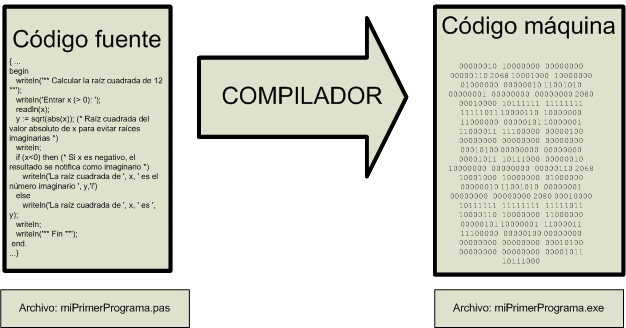
\includegraphics[width=0.65\textwidth]{Compilador.png}
	\end{SCfigure}

%Antecedentes
\textbf{Antecedentes}

\par{¿Sabías que, a mediados del siglo XIX, el profesor Charles Babbage de matemáticas e inventor en la universidad de Cambridge, Inglaterra, fue el primero en concebir la idea de un lenguaje de programación? Ada Lovelace es considerada como la primera programadora de la historia, ya que escribió los primeros programas para la máquina concebida por Babbage en tarjetas perforadas, siguiendo una lógica de programación muy similar a la empleada en nuestros días. Estos programas nunca pudieron verse ejecutados debido a que la máquina no fue construida \cite{garfinkel_shevtsov_guo_2017}.La tarjeta perforada (Ver Figura \ref{Imagen_2}) o simplemente tarjeta es una lámina hecha de cartulina que contiene información en forma de perforaciones según un código binario.} 
\\
%Imagen 2
\begin{SCfigure}[0.5][h]
	    \centering
		\caption{Tarjeta perforada, (Obtenido de: \href{https://mujeresconciencia.com/2018/06/27/tarjetas-para-programar-el-mundo/}{Mujeres con ciencia})}
		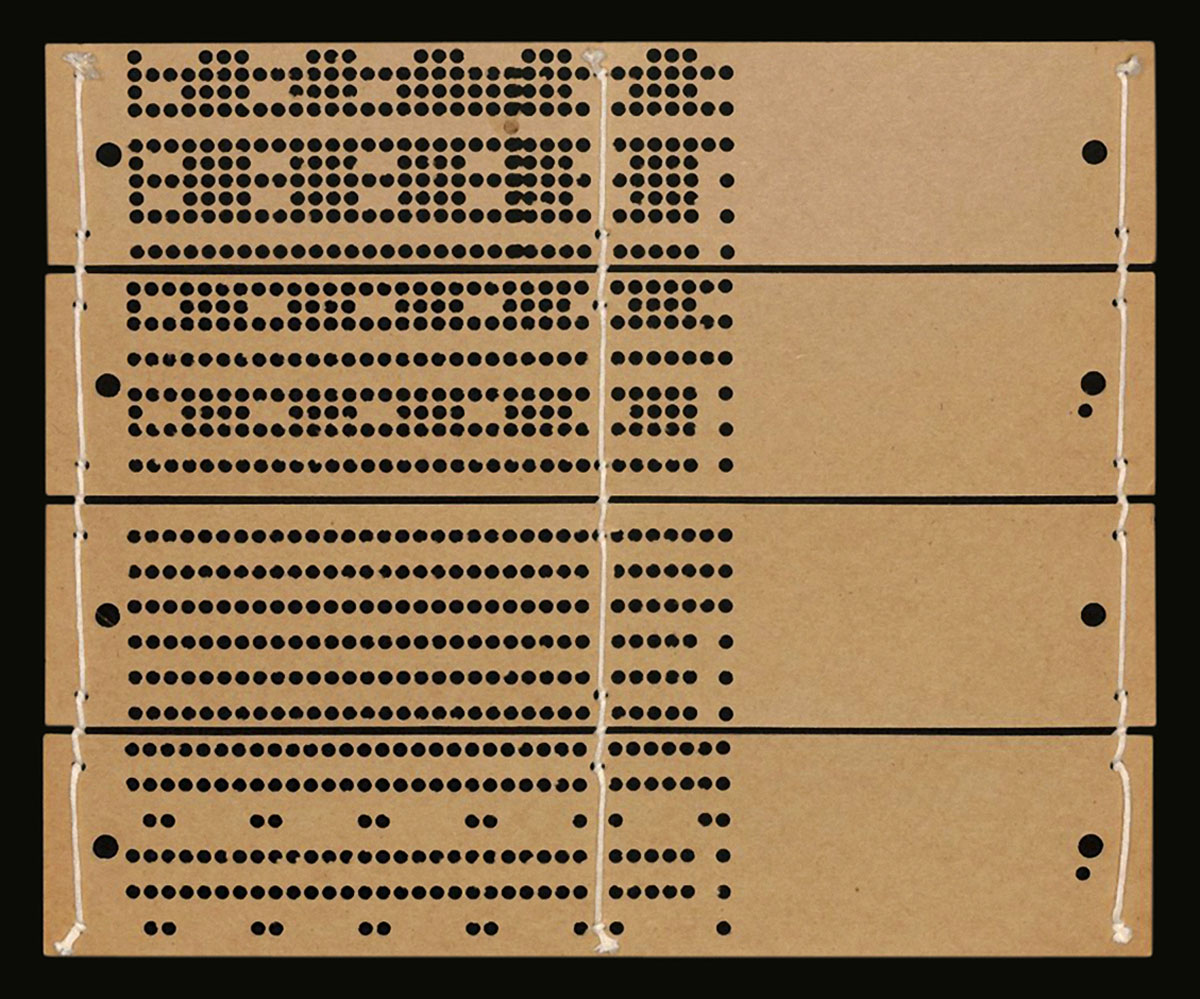
\includegraphics[width=0.5 \textwidth]{Tarjeta.jpg}
		\label{Imagen_2}
	\end{SCfigure}
	
	
	
\par{En 1823, con el apoyo del gobierno  británico, se aprobó el proyecto de construcción de una máquina diferencial. Esta máquina era un dispositivo mecánico diseñado para realizar sumas de forma repetitiva. Babbage abandonó el proyecto para dedicarse a su máquina analítica, influenciado por la creación de un fabricante de telas francés, Joseph Marie Jacquard, que había desarrollado una máquina tejedora, leyendo información codificada en tarjetas perforadas de papel rígido. Desde entonces, Babbage se propuso construir una máquina que efectuara cálculos matemáticos de precisión, empleando 20 dígitos, y que pudiera ser programada mediante tarjetas perforadas \cite{garfinkel_shevtsov_guo_2017}.}

\par{Aun cuando esta idea quedó sólo en el proyecto, fue una contribución muy importante para el diseño y funcionamiento de las computadoras actuales. Charles Babbage es considerado el padre de la informática. A pesar de que su máquina nunca pudo ser desarrollada, sus ideas y diseños sirvieron para la construcción y el progreso de las primeras computadoras modernas \cite{garfinkel_shevtsov_guo_2017}.}
\\ \\ 
%Clasificación
   \textbf{Clasificación}
   \par{Los circuitos microprogramables son sistemas digitales, trabajan con dos únicos niveles de tensión simbolizados con el cero (0) y el uno (1). Enseguida se muestran la clasificación de los tipos de lenguaje: }
   
   \begin{itemize}
       \item{Un lenguaje de programación de bajo nivel es el que proporciona poca o ninguna abstracción del microprocesador de una computadora. Es decir que hace referencia al código binario, esta orientado al hardware por lo tanto son instrucciones para el procesador. Con este tipo de lenguaje puedes construir sistemas operativos y núcleos}
       \item{Los lenguajes de programación de alto nivel se caracterizan porque su estructura semántica es muy similar a la forma como escriben los humanos, lo que permite codificar los algoritmos de manera más natural, en lugar de codificarlos en el lenguaje binario de las máquinas, o a nivel de lenguaje ensamblador.}
   \end{itemize} 
  
  
   %Tabla de ejemplos
    \begin{table}[h]
        \centering
        \resizebox{4.5 cm}{!} {
        \begin{tabular}{| c | c |}
            \hline
            Bajo nivel  & Alto nivel \\ \hline
            Assembly & C++ \\
            LOAD X      & Fortran \\
            ADD Y       & Java \\
            STORE Z     & PHP \\
            -           & Python \\
            -           & Perl \\ \hline
        \end{tabular}}
        \caption{Ejemplos}
   \end{table}
   
   
    %Tipos de programación
   \textbf{Tipos de programación}
   \begin{itemize}
       \item{\textbf{Programación lógica:} este tipo de programación se caracteriza por programar con relaciones e inferencia. Aquí el programador es responsable de especificar las relaciones lógicas básicas.}
       \item{\textbf{Programación funcional:}se caracteriza por programar con valores, funciones y formas funcionales (que son una relación entre una variable dependiente y una variable explicativa). Un programa funcional consiste en una expresión, llamémosla E, la cual es sujeto de unas reglas escritas. La reducción consiste en reemplazar alguna parte P de E por otra expresión P' según las reglas, este proceso se repite varias veces hasta que la expresión resultante no tenga parte que tengan que ser reescritas. La expresión obtenida de este proceso, E' es la que será la forma normal de E y es la salida del programa funcional.-H.P. Barendregt}
       \item{\textbf{Programación imperativa:} esta se caracteriza por programar con un estado y comandos que modifican ese estado. Tenemos dos partes importantes: imperativo, que es una orden o un comando, y el procedimiento, el acto, método de proceder, una manera de hacer algo. Cuando la programación imperativa se combina con otros subprogramas se le llama programación procedimental.}
       \item{\textbf{Programación concurrente:} se caracteriza por programar con más de un proceso. Este tipo de programación se utiliza para diseñado de compilado, algunos problemas son resueltos de forma natural usando un conjunto de procesos que operan al mismo tiempo, una solución secuencial que constituye sobre especificaciones y para reducir el tiempo de ejecución. Hay una diferencia entre operaciones secuenciales y concurrentes. Las secuenciales ocurren una después de otra mientras que las concurrentes son cuando ocurren al mismo tiempo.}
       \item{\textbf{Programación orientada a objetos:} este tipo de programación se caracteriza por programar con objetos, mensajes y jerarquías de objetos. Se enfoca en los datos de elementos pasivos definidos por relaciones o actos en funciones y procesos para elementos activos con su ambiente.}
   \end{itemize}
   %Lenguajes de programación
     \textbf{Algunos lenguajes de programación}
   \begin{itemize}
       \item{\textbf{C:} este tipo de lenguaje divide largos programas en pequeños módulos que son funciones y se enfoca en funciones y procesos que operan con datos. Se utiliza en tecnología de la información, ingeniería, administración, cuidado de la salud, procesamiento de imagen y programación de juegos. }
       \item{\textbf{C\#:} es un lenguaje de programación multiparadigma que cuenta con disciplinas fuertes de escritura, imperativa, declarativa, funcional, orientada a objetos. Se usa en tecnología de la información, ingeniería, diseño, control de calidad.}
       \item{\textbf{C++:} es un lenguaje orientado a objetos, es de medio nivel y es una extensión del lenguaje C. Se utiliza en tecnología de la información, ingeniería, diseño, control de calidad, administración, software, drivers firmware. }
       \item{\textbf{Python:} es un lenguaje de programación avanzado que es interpretado, orientado a objetos y construido en una flexible y robusta semántica. Es utilizado en desarrollo de Back-end, tecnología de la información, ingeniería, diseño, desarrollo web, frameworks, manejo de contenido avanzado, computación científica y numérica, gráficos de escritorio.}
       \item{\textbf{Ruby:} es un lenguaje de secuencias de comandos orientado a objetos y de código abierto que se puede utilizar de forma independiente o como parte del marco web de Ruby on Rails. Es utilizado en desarrollo, ingeniería de software, ingeniería en data science, desarrollo de WebApp, robótica, networkin, administración de sistema y seguridad.}
       \item{\textbf{PHP:}  es un lenguaje de secuencias de comandos de código abierto diseñado para crear páginas web dinámicas que funcionan de manera efectiva con bases de datos. También se utiliza como un lenguaje de programación de propósito general. Se usa para tecnología de la información, ingeniería, diseño, cuidado de la salud, finanzas, administración, desarrollo de aplicaciones Web, Scripting.}
       \item{\textbf{Java:} es un lenguaje de programación de alto nivel, orientado a objetos y de propósito general con varias características que lo hacen ideal para el desarrollo basado en web. Se utiliza en comunicación, educación, finanzas, ciencias de la salud, retail y utilidades, internet de las cosas, Cloud, videojuegos y apps móviles.}
       \item{\textbf{JavaScript:} es un lenguaje de programación del lado del cliente que se ejecuta dentro de un navegador cliente y procesa comandos en una computadora en lugar de un servidor. Normalmente se coloca en un archivo HTML o ASP. Se utiliza en tecnología de la información, ingeniería, diseño, marketing, finanzas, cuidado de la salud, desarrollo Front-end, desarrollo de juegos. Java y JavaScript no están relacionados}
   \end{itemize}
   \subsection{Potencia computacional y su importancia}
    
\par{Las supercomputadoras son máquinas computacionales masivas usadas para realizar cálculos complejos en una gran variedad de aplicaciones científicas. Dichas aplicaciones abarcan una amplia gama de tareas computacionales intensivas, incluidas la mecánica cuántica, la previsión meteorológica, la investigación climática, la exploración de petróleo y gas, la dinámica molecular y las simulaciones físicas, que requieren una cantidad de potencia informática y recursos que van más allá de lo que está disponible en general para servidores informáticos o estaciones de trabajo. Estas supercomputadoras se clasifican de acuerdo con su rendimiento según las operaciones de punto flotante por segundo (FLOPS). La medida de varias funciones indica, principalmente, el número de operaciones de este tipo que el procesador de hardware puede resolver en un segundo mezclando números pequeños, grandes e incluso fraccionarios. Este enfoque era muy costoso y limitaba el uso de supercomputadoras en unos pocos centros de investigación en todo el mundo. Para reducir los costos operativos y de adquisición, los investigadores comenzaron a construir supercomputadoras a partir de componentes comunes listos para usar (COTS, por sus siglas en inglés), como los que se usan en computadoras de escritorio y portátiles de uso general. Las supercomputadoras actuales constan de una multitud de nodos de cómputo interconectados a través de una red de alta velocidad. Cada nodo de cómputo cuenta con uno o más chips de procesador multinúcleo/multiproceso, varios módulos de memoria, uno o dos adaptadores de red y, posiblemente, algunos discos de almacenamiento local. Más recientemente, los aceleradores, en forma de unidades gráficas vectoriales o matrices de puertas programables en campo (FPGA), también se han abierto camino hacia la supercomputación convencional.}
 

\par{Por otro lado, los componentes COTS trajeron un nuevo conjunto de problemas que hace que las aplicaciones de informática de alto rendimiento (HPC) se ejecuten en un entorno hostil: 
\begin{itemize} 
\item Los componentes COTS son intrínsecamente más vulnerables que componentes de propósito especial y, debido a razones de costo, siguen diferentes procesos de producción y rutas de verificación que los sistemas integrados militares o industriales de misión crítica o mainframes de servidor. 
\item Los componentes COTS no están diseñados específicamente para resolver aplicaciones científicas y su rendimiento de un solo procesador era menor que el del procesador vectorial, por lo que generalmente se requiere una mayor cantidad de procesadores para lograr el rendimiento deseado. La combinación de una cantidad extremadamente grande de componentes del sistema aumenta en gran medida la probabilidad combinada de que al menos uno se rompa, experimente un error leve o deje de funcionar total o parcialmente. 
\item Se ha demostrado que las cargas de trabajo de HPC son extremadamente heterogéneas y posiblemente pueden estresar diferentes partes de las supercomputadoras, como la memoria, los procesadores o la red. Este comportamiento heterogéneo, a su vez, aumenta el estrés térmico y mecánico, reduciendo efectivamente la vida útil de cada componente y de todo el sistema. La ubicación y la instalación de la supercomputadora juega un papel importante en la resiliencia del sistema. Por ejemplo, estudios recientes confirman que las supercomputadoras instaladas en altitudes más altas, como Cielo en el Laboratorio Nacional de Los Álamos (LANL), están más expuestas a la radiación y muestran tasas de error leve más altas. 
\item El mero tamaño de las supercomputadoras actuales hace que sea imposible emplear soluciones de resiliencia comúnmente utilizadas en otros dominios, tanto por el costo como por razones prácticas. Las técnicas de resiliencia tradicionales, como la redundancia de módulo doble o triple (DMR, TMR), son prohibitivas en el contexto o grandes supercomputadoras debido a la gran cantidad de nodos de cómputo y componentes de nodos de cómputo. 
\end{itemize}
$Double-clickSelect

\par {A continuación se muestran las 10 mejores supercomputadoras:}
\begin{enumerate}[1.]
    \item Supercomputadora Fugaku
    %\itprocessesit
    \item Supercomputadora Sierra
    \item Sunway TaihuLight
    \item Perlmutter
    \item Selene
    \item Tianhe-2A
    \item Summit
    \item HPC5
    \item Frontier
\end{enumerate}






\newpage
\section{Herramientas bioinformáticas}
\par{Hoy en día existe un gran número de herramientas que pueden facilitar el desarrollo del modelado de sistemas. Esta sección muestra algunas herramientas que pueden ser útiles en el modelado de sistemas biológicos y pequeños ejemplos de cómo se pueden aplicar.}
    \subsection{Cello}
    \par{Cello es una herramienta que permite el diseño racional de circuitos genéticos que produzcan una señal de salida deseada a partir de una serie de datos de entrada. Cello automáticamente diseña una secuencia de ADN que codifica la señal de salida deseada a través de la especificación de sensores, actuadores y archivo de restricciones de usuario, lo que define el organismo, y válida las condiciones de operación. Todo esto se hace mediante el lenguaje de descripción de hardware Verilog, con el cual se crea un diagrama de circuito, asigna puertas, equilibra las restricciones para construir el ADN y simula el rendimiento. El resultado es una secuencia en la cual están implementados sistemas booleanos específicos según el organismo y así poder una predicción del funcionamiento del circuito.}
    \par{En 2016 el equipo de EPFL usó este software, en su página es posible encontrar cómo es que lo utilizaron, además de dar consejos en caso de que algún otro equipo busque información sobre su funcionamiento. Ellos mencionan como es posible aplicarlo en el proyecto sin saber el lenguaje de Verilog, el cuál puede ser un poco complicado si nunca se ha utilizado antes. Aquí se expone una manera de desarrollar en proyecto solamente con comandos arrastrables.}
    \par{Para más información hacer clic \href{https://2016.igem.org/Team:EPFL/Software_CELLO}{aquí}}
    \subsection{MATLAB}
    \par{MATLAB es una plataforma de programación para resolver problemas computacionales y matemáticos. Esta herramienta es un entorno cómodo que implica computación, visualización y programación, donde es posible expresar los problemas y sus soluciones de una forma similar a la matemática (\cite{gilat_2017}). Algunos de los usos más comunes de MATLAB son:}
    \begin{itemize}
        \item Cálculos matemáticos
        \item Creación de algoritmos
        \item Análisis de datos
        \item Creación de gráficas
        \item Modelado de sistemas
    \end{itemize} 
    \par{Una de las principales ventajas del uso de MATLAB es que es relativamente sencillo de usar y existen recursos en línea para aprender desde usos sencillos hasta usos más especializados \cite{Kirouac2019}. En la página de \href{https://la.mathworks.com/support/learn-with-matlab-tutorials.html}{MathWorks} se puede encontrar gran variedad de cursos gratuitos e interactivos para aprender a usar MATLAB.}
    \par{Además, MATLAB cuenta con una gran variedad de cajas de herramientas (Toolbox) que cuentan con propósitos específicos y facilitan el trabajo. Simbiology es Un ejemplo de cajas de herramientas muy útiles para el modelado de sistemas biológicos \cite{Park2019}.}
        \subsubsection{SimBiology}
        \par{Esta caja de herramientas permite modelar, simular y analizar diferentes sistemas biológicos \cite{Kirouac2019}. SimBiology facilita la creación de ecuaciones que describen el comportamiento de un sistema biológico al proveer un entorno gráfico dónde se puede construir un diagrama del sistema, definir parámetros y tipos de balances de materia \cite{Feigelman2016}.}
        \par{SimBiology cuenta con una gran variedad de facilidades para realizar modelos de fenómenos biológicos, esta herramienta cuenta con un amplio rango de solucionadores numéricos de simulaciones tanto estocásticas como  determinísticas \cite{Ullah2006}.}\\
        \par{\textbf{Ejemplo de modelado en SimBiology}}
        \par{Se muestra un ejemplo paso a paso del modelado de la unión de la histamina a su receptor y la competencia que viene de antihistamínicos.El ejemplo fue desarrollado con MATLAB versión 2020b.}
            \begin{enumerate}[1.]
                \item Abrir el entorno gráfico de SimBiology al escribir \textit{Simbiology} en la ventana de comandos.
                \item Crear un nuevo proyecto dando clic en la opción de \textit{Create New Blank Model} y darle un nombre.
                \item Añadir las especies (histamina, receptor de histamina y antihistamínico) y una reacción arrastrando los elementos dentro del compartimiento.
                \item Unir las especies a la reacción con Ctrl + Clic (La direccionalidad es muy importante).
                \item Definir concentraciones iniciales de cada una de las especies en el panel izquierdo.
                \item Marcar la reacción como reversible (dar clic en la reacción para que el panel aparezca) en el panel derecho y definir las constantes de reacción. 
                \item Guardar el modelo.
                \item Dar clic en \textit{Model Analyzer} y en la nueva ventana abrir el modelo que ya se construyó.
                \item En el botón \textit{Program} seleccionar \textit{Simulate model}, modificar las características en la que correrá la simulación y seleccionar el botón \textit{Run}.
            \end{enumerate}
    \subsection{Herramientas de modelado de proteína}
     \par{Muchos proyectos de biología sintética involucran proteínas. Comprender y predecir estas moléculas puede ayudar a comprender sistemas más complejos. También puede proporcionar información para diseñar experimentos. En consecuencia, dedicamos una sección a mostrar algunas de las herramientas que pueden ser útiles en el modelado de proteínas.}
    \subsubsection{I-TASSER}
        \par{I-TASSER es un servidor en línea que se puede utilizar para visualizar las posibles estructuras en la fusión de proteínas para que podamos tener información sobre su función. Las secuencias de aminoácidos se utilizan como entrada con estos. El servidor busca información en el Banco de Datos de Proteínas. Te envía plantillas de proteínas con plegamiento similar, con imágenes en 3D y una predicción de las propiedades de la proteína.}\\
        \par{\textbf{Ejemplo de uso I-TASSER}}
        \par{Se muestra un ejemplo de como utilizar este servidor para modelar una proteína}
            \begin{enumerate}[1.]
            \item Abrir la página de I-TASSER.
            \item Seleccionar en Online Services la pestaña de I-TASSER.
            \item Ingresar la secuencia de la proteína en formato FASTA o bien seleccionar el archivo en el cual se encuentra la secuencia.
            \item Ingresar la cuenta o bien crearla.
            \item Asignar un ID al trabajo para poder tener un mejor rastreo de tu secuencia.
            \item Esperar a que se tenga listo el modelado.
            \end{enumerate}
        \subsubsection{AlphaFold}
            \par{AlphaFold usa IA que puede predecir la estructura 3D de una proteína a partir de sus secuencias de aminoácidos \cite{Kiersten}. Alphafold predice secuencias a través de una red neuronal. Combina alineación de secuencias y características de proteínas homólogas para generar una estructura superior con precisión si lo comparamos con otras herramientas de predicción de proteínas \cite{DAVID}.}
            %Actualizar referencias con Bib.
        \subsubsection{Phyre \texorpdfstring{$^2$}{Lg}}
        \par{Phryre {$^2$}  por sus siglas en inglés es un motor de reconocimiento de homología/analogía de proteínas. Es la versión dos del servidor Phyre original, con nuevas actualizaciones y mejoras en su precisión y un rediseño más intuitivo y rápido de la interfaz del servidor. Esta herramienta nos sirve para modelar y predecir la estructura tridimensional (3D) de una o varias proteínas empleando una secuencias de proteínas o genes. También el modelado de la proteína basado en una estructura de plantilla proporcionada por el usuario, así como las proteínas multidominio. Para cumplir con este proceso, utiliza la alineación de modelos de Markov ocultos mediante HHsearch y así aumentar la precisión de la alineación y la tasa de detección \cite{Kelley_2017}.}  
        \par{Este cuenta con una biblioteca con información de nuevas estructuras agregadas, códigos PBD y homólogos cercanos. Asimismo, proporciona dos modos para modelar: el normal y el intensivo.}
            \par{\textbf{Normal:} Permite determinar la estructura de la proteína rápidamente pero aproximada.}
            \par{\textbf{Intensivo:} Permite determinar la estructura de la proteína más exacta pero el proceso es tardado.}
        \par{\textbf{Beneficios:}}
        \begin{itemize}
            \item Más longevidad en los resultados (1 mes).
            \item Permite visualizar y renovar trabajos anteriores.
            \item Imágenes listas para publicación.
            \item Creación de gráficas.
            \item Predice el sitio vinculante y la hélice transmembrana.
        \end{itemize}
        \par{\textbf{Extensiones:}}
        \par{Phryre {$^2$} 2 presenta una simulación de plegamiento ab initio llamada \textbf{Poing}, que ayuda a modelar secciones de la proteína sin homología detectable a través de estructuras conocidas. Para ello, Poing los asimila como resortes elásticos lineales y modela el módulo con su simulación física.}
        \par{\textbf{BackPhyre} es el inverso de Phyre; no predice la estructura 3D de una secuencia, pero basándose en la proteína, la compara con una estructura relacionada con un genoma de interés}
        \par{\textbf{Phyre Alarm} permite agregar una secuencia, escanearla de manera automática y comparar con la información nueva agregada a la biblioteca de pliegues (esta se actualiza semanalmente). Si la encuentra se notifican los resultados por correo electrónico.}
        \par{\textbf{Pasos para modelar:}}
            \begin{enumerate}[1.]
            \item Buscar en tu navegador Phyre 2. 
            \item Registrarse en la plataforma.
            \item Confirmar tu e-mail.
            \item Llenar los datos requeridos en blanco: e-mail y secuencia de aminoácidos. \textbf{Tip:} Si tienes más de 5 o 6 secuencias para modelar utilizar la opción “Batch”, disponible en el Modo experto después de iniciar sesión. 
            \item Seleccionar el modo: normal o intensivo.
            \item Seleccionar el propósito de utilizar el servidor: no lucrativo, lucrativo u otro.
            \item Dar clic en “Phyre Search”.
            %\begin{figure}
                   
            %\end{figure}
            \item Esperar, el tiempo de espera depende del largo de tu secuencia.
            \item Los resultados serán enviados al correo.
            %\begin{figure}
                   
            %\end{figure}
            \end{enumerate}

        \subsubsection{PyMOL}
        \par{PyMOL es un sistema de visualización molecular para analizar y compartir datos moleculares basado en el software Python que interpreta más de 30 formatos de archivo e incluso admite scripts personalizados. Gracias a una nueva interfaz de usuario unificada, es posible crear rápida y fácilmente películas a través de un paisaje molecular, contando transformar estructuras de proteínas con diferentes texturas y animar trayectorias con varios efectos de movimiento. De manera similar, puede personalizar el gráfico codificando segmentos o cambiando los colores de las cadenas \cite{Yuan_2017}.}
        \par{\textbf{Beneficios:}}
            \begin{itemize}
                \item Sistema rápido y no pesado.
                \item Imágenes de buena calidad.
                \item Incluye fragmentos prediseñados.
                \item Personalización.
                \item Se pueden activar o ocultar elementos.
            \end{itemize}
            \par{\textbf{Extensiones:}}
            \par{Con \textbf{AxPyMol} se pueden insertar datos moleculares interactivos y visualizarlos.}
       
    \subsection{Herramientas de simulación de interacciones moleculares}
\subsubsection{UCSF Chimera}
\par{Chimera es un programa multifuncional que permite el acoplamiento molecular entre proteínas y ligandos pequeños de archivos .pdb (Banco de datos de proteínas). Además, este programa permite la visualización y análisis de las estructuras a través de mapas de densidad y alineación de secuencias. Además permite el color de las cadenas de las proteínas y muestra las interacciones entre proteína-enlace.}
\begin{SCfigure}[0.65][ht]
	    \centering
		\caption{Visualización compleja de enlaces de proteínas en Chimera  \cite{Pettersen_2004}}
		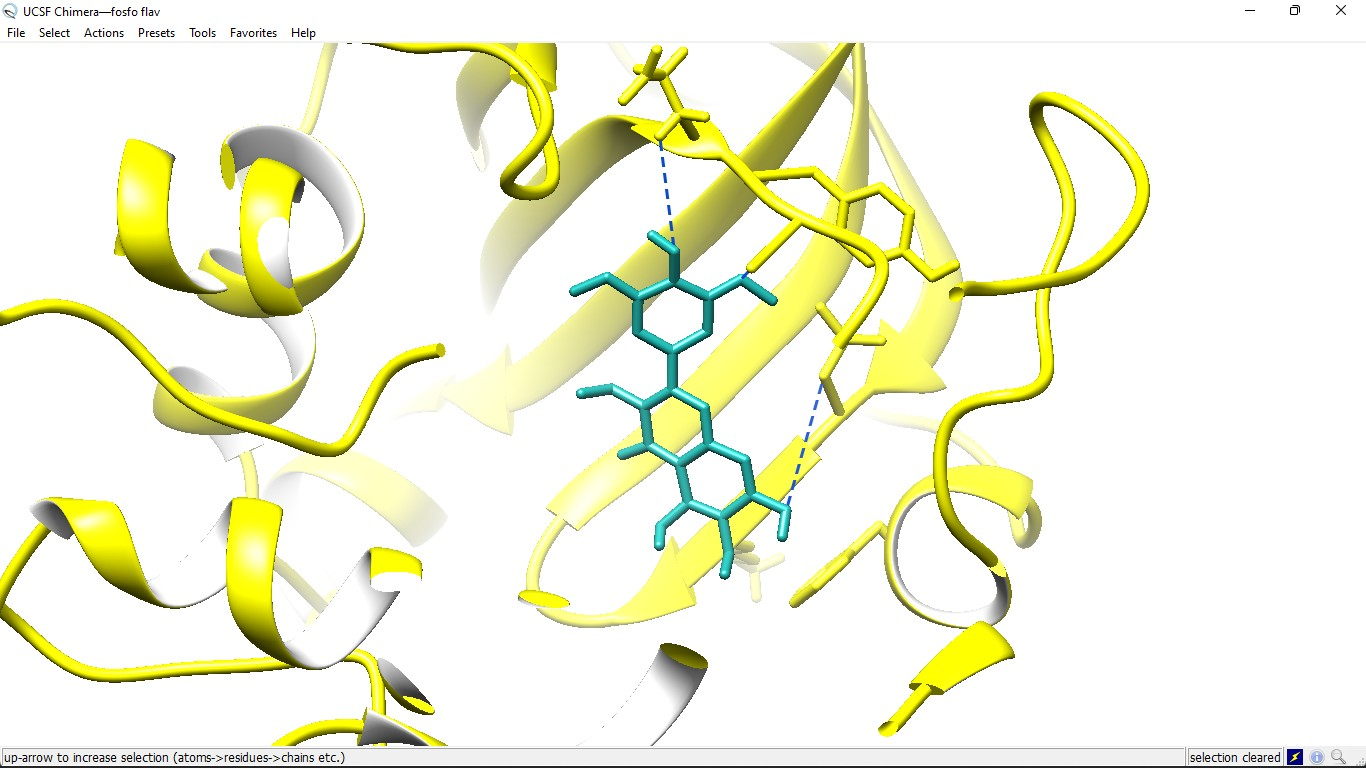
\includegraphics[width=0.65\textwidth]{chimera}
	\end{SCfigure}

\par{\textbf{Paso por paso}}
\par{A continuación se muestran los siguientes pasos básicos de cómo acoplar con este programa:}
    \begin{enumerate} [1.]
        \item Una vez que tenga su proteína y ligando, abra el programa USCF Chimera.
        \item{Luego abra sus archivos en el programa. Será necesario sumar los estados de protonación y la asignación de cargas.}
        \item{Guarda los archivos previamente cargados y protonados con extensión .mol2.}
        \item{Ejecute el acoplamiento molecular a través de AutoDock Vina.}
        \item{Guarda las poses obtenidas con la extensión .pdb.}
    \end{enumerate}
\subsubsection{ArgusLab}
    \par{ArgusLab es un programa de licencia libre con una interfaz gráfica fácil de usar. Es un visor y editor de estructuras biológicas o moléculas orgánicas y permite hacer acoplamiento molecular. La ventaja de ArgusLab, sobre otros programas de su tipo, es que incorpora parámetros de campos de fuerza para varios metales como Ni, Cu, Ti, Co, Mn y más. De esta manera, la diversidad de ligandos y receptores puede estudiarse mediante estudios de acoplamiento molecular.}
\begin{SCfigure}[0.65][ht]
	    \centering
		\caption{Visualización compleja de enlaces de proteínas en ArgusLab  \cite{Thompson_2004}}
		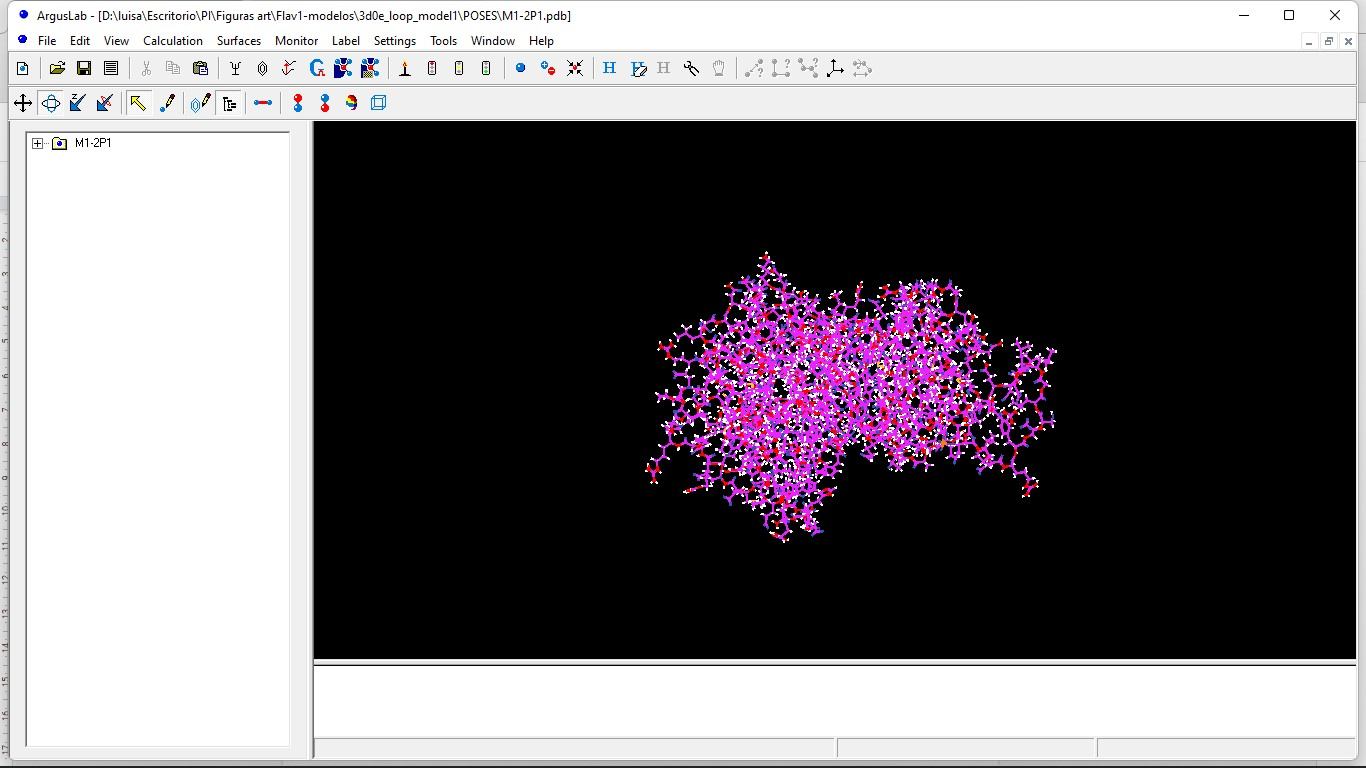
\includegraphics[width=0.65\textwidth]{argus}
	\end{SCfigure} 
 \par{\textbf{Paso a paso}}
 \par{A continuación se muestran los siguientes pasos básicos para considerar cómo acoplar con este programa:}
 \begin{enumerate}[1.]
     \item Una vez que tenga su proteína y ligando, abra el programa ArgusLab.
     \item Abre tus archivos en el programa.
     \item Elimine las moléculas de agua presionando Mayús + clic en la última molécula de agua/clic derecho/eliminar.
     \item Seleccione los aminoácidos del sitio de unión y haga un grupo con ellos. Luego haz lo mismo con tu ligando.
     \item Ejecute el acoplamiento molecular con la opción Calculation/Dock a Ligand.
     \item Guarde los resultados en la extensión .pdb.
     \end{enumerate}

\subsubsection{PyRx}
\par{PyRx es un programa que permite el acoplamiento molecular entre proteínas y pequeños enlaces a través de AutoDock Vina. Además, puede tener una visualización básica de las moléculas.}

\begin{SCfigure}[0.65][ht]
	    \centering
		\caption{Visualización compleja de enlaces de proteínas en PyRx
            \cite{Dallakyan_2014}}
		      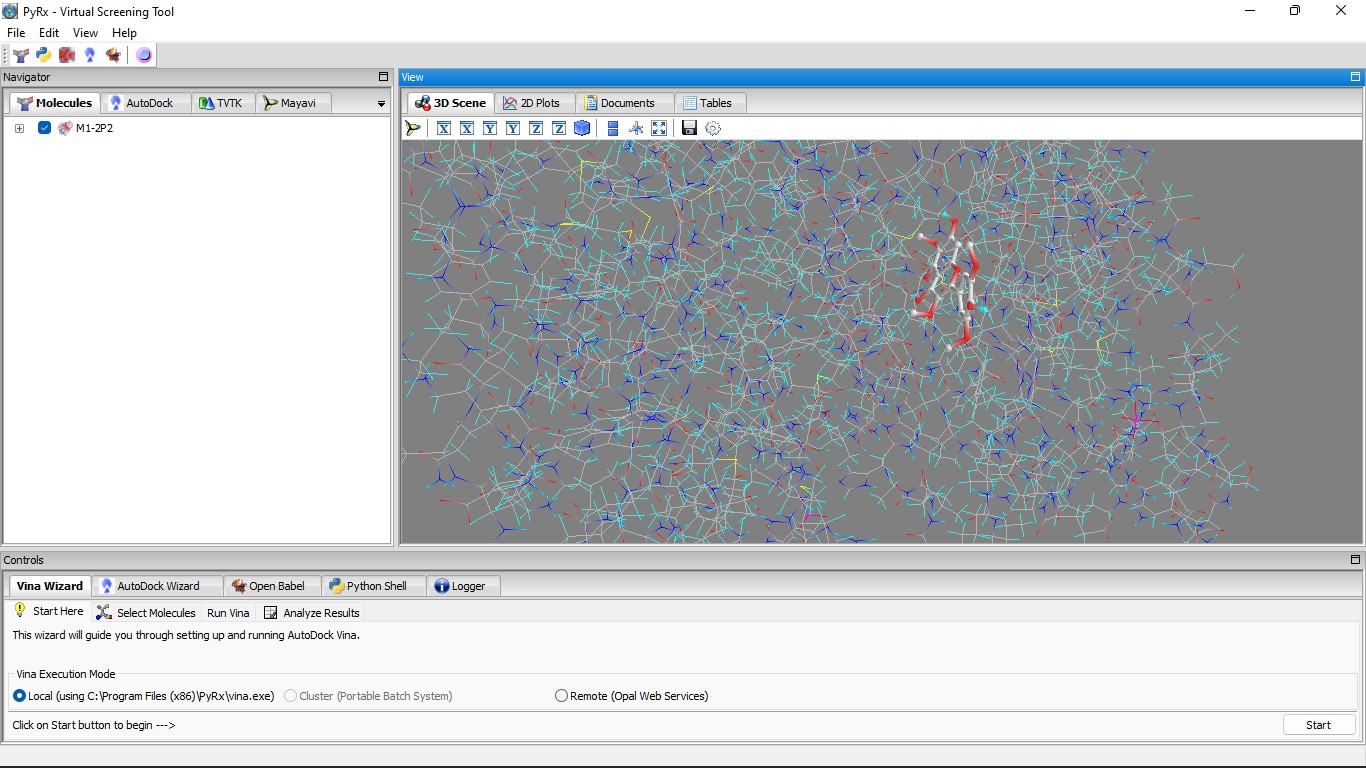
\includegraphics[width=0.65\textwidth]{pyrx.jpg}
	    \end{SCfigure}

    \par{\textbf{Paso a paso:}}
    \par{A continuación se muestran los siguientes pasos básicos de cómo acoplar con este programa:}
    \begin{enumerate}[1.]
        \item Una vez que tenga su proteína y ligando, abra PyRx.
        \item Abra sus archivos en el programa en la sección AutoDock/Vina Wizard.
        \item Establezca las condiciones de la caja de acoplamiento molecular.
        \item Ejecute el acoplamiento molecular.
        \item Los resultados en extensión .pdb.
    \end{enumerate}

 \subsubsection{Swiss-Model}
    \par{Swiss-Model es un servidor de modelado de homología de estructuras de proteínas totalmente automatizado, accesible a través del servidor web Expasy o el programa DeepView (Swiss Pdb-Viewer). El propósito de este servidor es hacer que el modelado de proteínas sea accesible para todos los investigadores de ciencias de la vida en todo el mundo.}

    \par \textbf{Paso a paso}:
\begin{enumerate}
    \item Selección de la proteína molde.
    \item Debe ser seleccionado como la mejor plantilla. Los criterios para elegir la estructura utilizada como referencia siguen siendo los mismos que en los pasos del MODELLER. Preste atención al valor de identidad ($>$ 25\%) entre las secuencias, la mejor cobertura, el valor E bajo y la mejor resolución cristalográfica (cuanto más pequeño, mejor).
    \item Alineación y construcción de modelos.
    \item SWISS-MODEL ya trabaja internamente en la alineación. Solo necesita seleccionar el modelo de la lista de selección dada, y el servidor obtiene el archivo PDB. Luego, el modelo se construye en función de la plantilla y la alineación después de hacer clic en Construir modelos. Podemos ver que SWISS-MODEL elimina automáticamente la región del péptido señal y no permite la inserción del péptido señal.
    \item Evaluación del modelo
    \par{SWISS-MODEL tiene sus herramientas de evaluación. Para evaluar el modelo debemos prestar atención a los valores de QMEAN (Qualitative Model Energy Analysis) y GMQE (Global Model Quality Estimation). QMEAN es un estimador conocido como puntuación z. Cuando el valor z es cercano a cero, significa que el modelo se considera confiable. Por lo tanto, existe una buena concordancia entre el modelo y las estructuras experimentales de tamaño similar. Las propiedades geométricas proporcionan una estimación de la calidad absoluta general. El GMQE, por otro lado, está en un rango de 0 a 1. Cuanto más alto es, más preciso es el modelo para la cobertura y la alineación del modelo objetivo. SWISS-MODEL también proporciona un gráfico de Ramachandran interactivo en la página web. El estadístico de parcela de Ramachandran es el 96,72\% de los residuos en regiones favorables. Después de descargar el modelo, se puede realizar una comparación visual entre la plantilla y las estructuras del modelo mediante la alineación estructural con la herramienta PyMOL.}
\end{enumerate}

\subsubsection{CHARMM-GUI}
\par{Entre varias herramientas de modelado basadas en la web, CHARMM-GUI, [http://www.charmm-gui.org], se propone simplificar y generalizar los protocolos para construir sistemas de simulación complejos y preparar archivos de entrada de simulación para paquetes de simulación ampliamente utilizados, como CHARMM, NAMD, GROMACS, AMBER, GENESIS, LAMMPS, Desmond, OpenMM y CHARMM/OpenMM para facilitar el uso de técnicas de simulación habituales y avanzadas \cite{Jo_2017}.}
\par{Desde su desarrollo en 2006, CHARMM-GUI se ha expandido a una gama de capacidades y ahora contiene varios módulos diferentes diseñados para configurar una amplia gama de sistemas biológicos (Fig. 1) \cite{Jo_2017}}.

\par El workflow implementado en el servidor HDOCK se muestra en la Figura 8.
        \begin{SCfigure}[0.65][ht]
	    \centering
		\caption{Vista esquemática de los módulos en el generador de entrada CHARMM-GUI. [La figura en color se puede ver en willeyonlinelibrary.com]\cite{Jo_2017} )}
		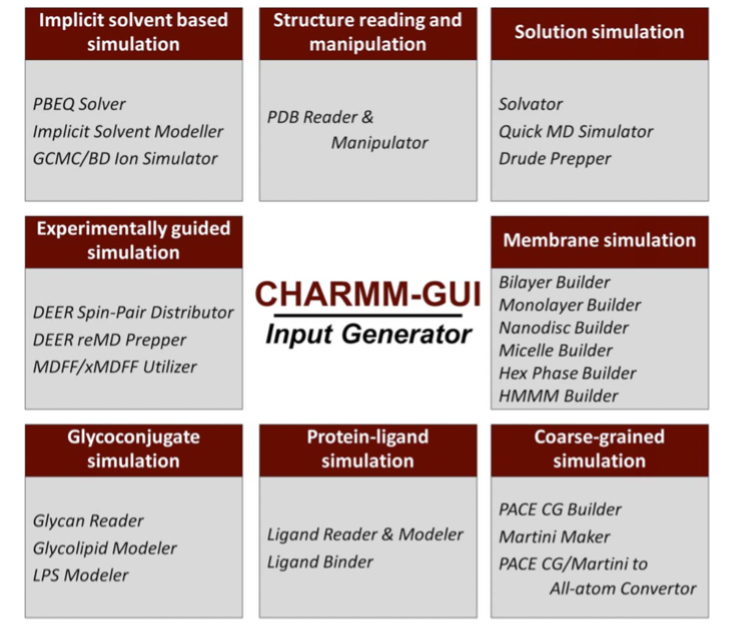
\includegraphics[width=0.65\textwidth]{images/Imagen 1.png}
	\end{SCfigure}\textbf{}

    \par{La filosofía en el desarrollo de CHARMM-GUI no se trata solo de proporcionar los elementos esenciales del modelado molecular, sino también de ayudar a los usuarios a realizar una tarea. Por ejemplo, construir un sistema de membrana o disolver una proteína agregando una interfaz optimizada hará que CHARMM-GUI sea accesible para usuarios con menos experiencia en herramientas de modelado y, sin embargo, útil para expertos, especialmente para la generación de sistemas por lotes \cite{Jo_2017}.}

    \par{Una limitación crucial es que CHARMM-GUI contiene muchos parámetros predeterminados (p. ej., la cantidad de pasos para minimizar o los detalles de cómo disolver una proteína), que están ocultos para los usuarios y pueden hacer que CHARMM-GUI sea menos atractivo para los usuarios más avanzados. sus necesidades específicas de personalización \cite{Jo_2017}}

    \subsubsection{HDOCK}
    \par{Las proteínas y los ácidos nucleicos son los dos tipos más importantes de macromoléculas biológicas en la célula. Sus interacciones son cruciales para muchos procesos biológicos como la transducción de señales, la regulación celular, la síntesis de proteínas, la replicación y reparación del ADN, la transcripción del ARN, etc. Por lo tanto, la determinación de sus estructuras complejas es valiosa para comprender el proceso biológico a nivel atómico y así desarrollar terapias. intervenciones o medicamentos dirigidos a estas interacciones. Dado el alto costo y las dificultades técnicas de los métodos experimentales, el acoplamiento molecular, que predice computacionalmente la complejidad de las estructuras individuales, ha desempeñado un papel importante en la determinación de la disposición compleja \cite{Yan_2017}. Para hacer un uso automático en lo que respecta a la información vinculante del PDB en el muelle, HDOCK es un servidor web útil.}
    
    \par{El servidor HDOCK (http://hdock.phys.hust.edu.cn/) es un seguimiento altamente integrado de búsqueda de homología, modelado basado en plantillas, predicción de estructuras, acoplamiento macromolecular, información biológica, gestión de trabajos para proteínas robustas y rápidas. acoplamiento de proteínas. Se distingue por el uso de secuencias de aminoácidos como entrada y una estrategia de acoplamiento híbrido donde la información experimental (sobre el sitio de unión proteína-proteína) y la dispersión de rayos X de ángulo pequeño se pueden incorporar durante los procesos de acoplamiento y post-acoplamiento. El servidor también admite el acoplamiento de proteína-ARN/ADN con una función de puntuación intrínseca. Proporciona la plantilla y los modelos de unión basados en acoplamiento de dos moléculas y permite la descarga de visualización interactiva. El servidor HDOCK se usa y ha procesado más de 30 000 trabajos de acoplamiento desde su lanzamiento oficial en 2017. Normalmente, el servidor puede completar un trabajo de acoplamiento en 30 minutos}

    \par{El flujo de trabajo implementado en el servidor HDOCK se muestra en la Figura 9.}
    \begin{SCfigure}[0.65][ht]
	    \centering
		\caption{El flujo de trabajo del servidor web HDOCK se divide en cuatro etapas: (1) entrada de datos, (2) búsqueda de similitud de secuencia, (3) modelado de estructuras y (4) acoplamiento global basado en FFT en el que se da prioridad a las estructuras de entrada del usuario . \cite{Yan_2017})}
		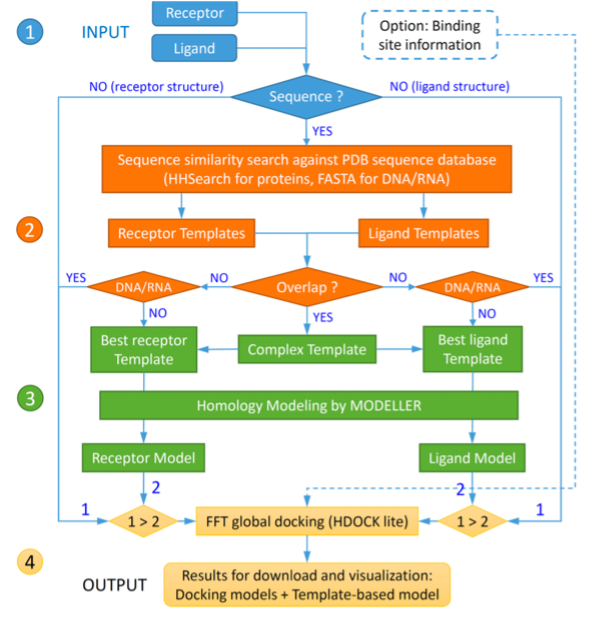
\includegraphics[width=0.65\textwidth]{Imagen 2.png}
	\end{SCfigure}\textbf{}

\par{Según \cite{Jo_2017} para facilitar mejor el uso del servidor HDOCK por parte de usuarios normales, especialmente para usuarios no expertos, el servidor está diseñado para aceptar entradas de secuencia y estructura para proteínas, dos para estructuras y dos para secuencias, como sigue:
1) Cargue su archivo pdb en formato PDB.
2) Proporcione su archivo pdb en PDB ID: ChainID (por ejemplo, 1CG1: E).
3) Copie y coloque la secuencia de proteína posterior al acoplamiento a continuación en formato FASTA.
4) Cargue su archivo de secuencia de proteínas en formato FASTA.}

\subsubsection{GLYCAM-Web}
Muchas áreas de investigación basadas en el acoplamiento centradas en los aspectos estructurales de las biomoléculas "trasladadas al ciberespacio" en los últimos 20 a 30 años se han vuelto aún más prominentes. Amplificado por la mayor accesibilidad del espacio (desde dispositivos móviles hasta la nube) y recursos aún más sofisticados y potentes disponibles para la informática de alto rendimiento. La glicobiología estructural se ha beneficiado enormemente de este progreso y ha aprovechado las herramientas y recursos computacionales desarrollados específicamente para el análisis estructural de carbohidratos \cite{Yuriev_2015}.
GLserverWeb apunta a la predicción de carbohidratos tridimensionales y estructuras macromoleculares, incluidos los carbohidratos.
El servidor es creado y operado por el grupo de investigación del Prof. Robert J. Woods en el Centro de Investigación de Carbohidratos Complejos (CCRC) en la Universidad de Georgia, Atenas. Este servidor puede realizar modelado conformacional de oligosacáridos contando el modelado 3D de glicoproteínas.
Es fundamental mencionar que:
1. El generador de carbohidratos, que incluye un generador crucial para los glicosaminoglicanos (GAG),
2. el constructor de glicoproteínas,
3. y las bibliotecas de oligosacáridos son archivos adjuntos relevantes para modelar la conformación de oligosacáridos. El servidor es fácil de usar y permite una variedad de opciones de carga y descarga.
Dado que ya existe una variedad de formatos de archivo, específicos del programa que se utilizan en el modelado molecular, la facilidad de uso relacionada con la portabilidad de los formatos de archivo es una característica importante de "bienes raíces" muy valorada por los habitantes del ciberespacio \cite.

\subsection{Herramientas de simulación de interacciones moleculares}
\subsubsection{GROMACS}
    \par{GROMACS es un programa multiplataforma de código abierto para realizar simulaciones de dinámica molecular y minimización de energía de sistemas con cientos de millones de partículas. Permite conocer y predecir el comportamiento de propiedades macroscópicas a través de la descripción de sistemas químicos complejos en términos de un modelo atómico realista.}
    \par{Revisando un pequeño ejemplo \cite{Villa_2017}, veremos la visualización de una pequeña proteína (Factor Xa, código PDB:v1FJS), que es una proteína que genera coágulos sanguíneos. Para visualización:}
    \\
    \par{importar nglview como ng}
    \par{$view = ng.show_structure_file("input/1fjs.pdb")$}
    \par{Vista}
    \\
    \par{De esta manera podemos ver una imagen como la de la Figura 3.}
\begin{SCfigure}[0.65][ht]
	    \centering
		\caption{Visualización del factor Xa(De: \cite{Villa_2017})}
		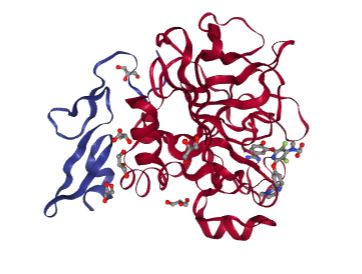
\includegraphics[width=0.65\textwidth]{Proteina.JPG}
	\end{SCfigure}
\par{Sin embargo, esta visualización contiene átomos que no corresponden a la estructura de la proteína. Para eliminar estos átomos (llamados "HETATM" en el archivo PDB), es cuestión de usar grep:}
\vspace{0.5 cm}

\par{$!grep -v HETATM input/1fjs.pdb > 1fjs_protein_tmp.pdb$}
\par{$!grep -v CONECT 1fjs_protein_tmp.pdb > 1fjs_protein.pdb$}
\par{Para visualizarlo:}
\par{Importar nglview como ng}
\par{$view = ng.show_structure_file("1fjs_protein.pdb")$}
\par{Vista}
\par{Así obtenemos una estructura más pura como en la Figura XXX:}
\begin{SCfigure}[0.65][ht]
	    \centering
		\caption{Visualización pura del factor Xa (De\cite{Villa_2017})}
		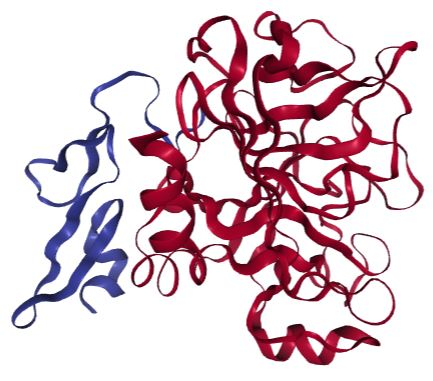
\includegraphics[width=0.5\textwidth]{ProteinaPura.JPG}
	\end{SCfigure}

\subsubsection{AutoDocks}
\par{Autodock es uno de los software de simulación de modelos moleculares más utilizados, diseñado para predecir la unión entre moléculas pequeñas y receptores con estructuras tridimensionales conocidas. Los cálculos realizados se desarrollan en 4 pasos principales:}
\vspace{0.4 cm}

\par{Elaboración de expedientes de coordenadas.
Durante esta etapa, el ligando y el receptor pueden incluir la información necesaria para usar AutoDock. Para ello se utilizan archivos tipo PDBQT que incluyen átomos de hidrógeno polares, cargas parciales, tipos de átomos e información sobre la flexibilidad de las moléculas. Para generar archivos es posible utilizar AutoDockTools.}
\par{Ejecutando AutoGrid.
 La ejecución de AutoDock requiere un mapa de cuadrícula precalculado para cada tipo de átomo en el ligando de acoplamiento. Estos mapas consisten en una red tridimensional de puntos espaciados regularmente que rodean una región de interés en la macromolécula que se ha estudiado. Para iniciar AutoGrid, se utiliza el siguiente código:}

\vspace{0.4 cm}
    autogrid4 -p macro.gpf [-l macro.glg]
\vspace{0.4 cm}
\par{Acoplamiento molecular con AutoDock. AutoDock evalúa las interacciones proteína-ligando en cada punto mediante una simulación de grupos. Para esto, AutoDock requiere un mapa calculado por AutoGrid, un ligando en formato PDBQT y un archivo de parámetros para la agrupación. Los cálculos comienzan con el siguiente código:}
\vspace{0.4 cm}

autodock4 [-i][-u][-t] -p lig.dpf [-l lig.dlg]

\vspace{0.4 cm}

\par{Evaluación de resultados.
Al final de la simulación, se obtienen las coordenadas de cada punto donde se formó la unión. Luego, la información sobre la formación de cúmulos y energías de interacción. El procesamiento de datos se realiza en la sección "Analizar" en el menú AutoDockTools.}
\newpage

\subsubsection{ClusPro}

\par{El servidor ClusPro es usado para el análisis estructura de un acoplamiento proteína-proteína y los resultados obtenidos permiten la identificación de las mejores conformaciones de acoplamientos moleculares. ClusPro cuenta con una interfaz de usuario básica, pero también permite aplicar varias opciones avanzadas en la búsqueda, como eliminar regiones de proteínas no estructuradas, aplicar atracción o repulsión, tener en cuenta las restricciones de distancia por pares, construir homomultímetros y localizar sitios de unión a heparina. (Kozakov et al., 2017). La ejecución de los análisis en el servidor se realiza siguiendo tres pasos computacionales (Kozakov et al., 2017):} 

\begin{enumerate}
    \item Ajuste de cuerpo rígido mediante el muestreo de miles de millones de conformaciones;
\item Agrupamiento basado en la raíz de la desviación cuadrática media (RMSD) de las 1.000 estructuras de energía más bajas generadas, para encontrar los cúmulos más grandes que representarán los modelos más probables del complejo;
\item Refinamiento de estructuras seleccionadas mediante minimización de energía
\end{enumerate}
\subsubsection{PIPER}
\par{ PIPER es un programa de ajuste basado en el enfoque de correlación de la transformada rápida de Fourier (FFT) y se utiliza en el paso de ajuste del cuerpo rígido. Una proteína receptora se coloca en el origen del sistema de coordenadas en una cuadrícula fija, mientras que un ligando-proteína se coloca en una rejilla móvil. En este proceso, la energía de interacción se escribe en forma de una función de correlación y el algoritmo basado en FFT permite el ajuste de proteínas sin información previa sobre la estructura del complejo (Kozakov et al., 2017).}
\subsubsection{PatchDock}
\par{PatchDock utiliza una técnica similar a un rompecabezas. Dadas dos moléculas, sus superficies se dividen en piezas de acuerdo con la forma de la superficie. Estas piezas corresponden a patrones visualmente distinguibles. Una vez que se identifican los fragmentos, se pueden superponer utilizando algoritmos de forma coincidente. El algoritmo tiene tres etapas principales:}
\begin{enumerate}
    \item Representación de la forma molecular: en este paso, se calcula la superficie molecular de la molécula. A continuación, se aplica un algoritmo de segmentación para detectar manchas geométricas (piezas de superficie cóncava, convexa y plana). Las piezas se filtran de modo que solo se retienen las piezas con residuos de puntos calientes.
    \item Coincidencia de fragmentos de superficie: un híbrido de las técnicas de emparejamiento Geometric Hashing y Pose-Clustering son trozos de ligando-proteína detectados en el paso anterior. Los trozos cóncavos se combinan con trozos convexos y los planos con cualquier tipo de trozos.
    \item Filtrado y puntuación: se examinan los complejos candidatos del paso anterior. Todos los complejos con penetraciones inaceptables desde los átomos receptores hasta los átomos ligandos son descartados. Finalmente, los candidatos restantes se clasifican de acuerdo con una puntuación de complementariedad de forma geométrica.
\end{enumerate}
\par{Los resultados de PatchDock se presentan en una lista con los complejos receptor-ligando candidatos. La lista se presenta al usuario en un formato de tabla, cada fila de tabla representa un complejo candidato.}
\par{Los parámetros utilizados son:}
\begin{itemize}
    \item\textbf{Solución No:} Número del candidato complejo.
    \item \textbf{Puntuación:} Puntuación de complementariedad de la forma geométrica. Los complejos candidatos se ordenan de acuerdo con esta puntuación.
    \item \textbf{Área:} Área de interfaz aproximada del complejo.
    \item\textbf{ECA (ACE en inglés):} Energía de contacto atómico.
    \item \textbf{Transformación 3D:} 3 ángulos de rotación y 3 parámetros de traslación. La transformación se aplica a la molécula de ligando.
    \item \textbf{Documento PDB del complejo:} La estructura compleja prevista en formato PDB.
\end{itemize}
\subsubsection{FireDock}
\par{ Como cualquier otro software para el análisis y puntuación de soluciones de acoplamiento proteína-proteína, FireDock utiliza dos opciones para la entrada inicial en su servidor: un archivo de transformación, que requiere una entrada de las moléculas receptoras y de ligando y los archivos de transformación, siguiendo el formato de rotaciones y traslaciones en los ejes X, Y y Z; o con un archivo modelo,  que utiliza un archivo que contiene modelos de los complejos para el análisis y de las cadenas de receptores y ligandos. La salida para obtener los resultados,por lo tanto, sigue la tabla del modelo con todas las soluciones de entrada, clasificadas por el valor de energía global, y que tiene varios parámetros de puntuación, a saber:}

\begin{itemize}
    \item Rango: relacionado con la energía general; 
    \item Número de solución: relacionado con el orden de las transformaciones o modelos; 
    \item Energía global: la energía vinculante de la solución; 
    \item Las fuerzas atractivas y repulsivas de Van der Waals (VdW) y su contribución a la energía de unión general;
    \item Energía de contacto atómico (ECA) en relación con la energía de enlace global. 
    \item La contribución de los puentes de hidrógeno (HB) a la energía de unión general.
\end{itemize}
   
 \subsubsection{PyDock}
    \par{PyDockWEB es un servidor web para la predicción de acoplamiento de cuerpo rígido de estructuras complejas proteína-proteína utilizando una nueva versión del algoritmo de puntuación pyDock. Utilizamos aquí una nueva implementación FTDock paralela personalizada, con tamaño de cuadrícula ajustado para cálculos FFT óptimos, y una nueva versión de pyDock, que acelera drásticamente los cálculos manteniendo la misma precisión predictiva. Dadas las coordenadas 3D de dos proteínas que interactúan, pyDockWEB devuelve las mejores orientaciones de acoplamiento obtenidas principalmente por la electrostática y la energía de desolvatación.}
    \par{El servidor PyDockWEB es una aplicación web para el uso del programa de acoplamiento y puntuación proteína-proteína pyDock. Los usuarios pueden enviar fácilmente trabajos de pyDock para ser ejecutados en un proceso de cinco pasos a través de un Front-end fácil de usar. En el primer paso, los usuarios deben introducir un nombre de proyecto y una dirección de correo electrónico de notificación. En el segundo paso, se selecciona el algoritmo de puntuación. En el tercer paso, los usuarios pueden cargar sus archivos de coordenadas de proteínas o indicar el código PDB, en cuyo caso, los archivos PDB se descargarán automáticamente del Banco de Datos de Proteínas RCSB. En ambos casos, los archivos PDB se analizan automáticamente para seleccionar las cadenas de receptores y ligandos disponibles. También está disponible una opción para configurar automáticamente un trabajo de acoplamiento con archivos PDB de ejemplo. En el cuarto paso, los usuarios pueden especificar restricciones de distancia opcionales, que se calcularán utilizando el módulo pyDockRST. Finalmente, en el quinto paso, los usuarios verificarán si los datos proporcionados son correctos y enviarán un trabajo de acoplamiento a la fila del servidor. Después del envío del trabajo, el usuario es redirigido a una página web donde el estado del proyecto se actualiza automáticamente y los archivos de resultados se pueden descargar una vez finalizado el cálculo. En esta página web, los 10 mejores modelos puntuados por PyDock se muestran utilizando Jmol.}
\begin{itemize}
    \item  \textbf{Parámetros:} Electrostática, Desolvatación, VdW (Van der Waals)
\end{itemize}
   
    \par{El esquema se basa en electrostática coulombica con una constante dieléctrica dependiente de la distancia, y energía de desolvatación implícita con parámetros de solvatación atómica previamente ajustados para el acoplamiento proteína-proteína de cuerpo rígido. Esta función de puntuación no depende en gran medida de la geometría específica de las posturas de acoplamiento y, por lo tanto, se puede utilizar en conjuntos de acoplamiento de cuerpo rígido generados por una variedad de métodos. Hemos probado el procedimiento en un gran conjunto de referencia de 80 casos de acoplamiento sin consolidar. El método es capaz de detectar una solución casi nativa a partir de 12.000 posturas de acoplamiento y colocarla dentro de las 100 soluciones de acoplamiento de menor energía en el 56\% de los casos, de una manera completamente sin restricciones y sin ninguna otra información adicional. Específicamente, una solución casi nativa se ubicará dentro de las 20 mejores soluciones en el 37 \% de los casos. La simplicidad del enfoque permite una mejor comprensión de los principios físicos detrás de la asociación proteína-proteína, y proporciona una herramienta rápida para la evaluación de grandes conjuntos de posturas de acoplamiento de cuerpo rígido en busca de la orientación casi nativa.}

\subsection{Parámetros usados en modelado}
\par{En el modelado estructural, hay varios parámetros utilizados por diferentes programas para expresar matemáticamente qué tan cerca está su resultado de la estructura de la proteína. También son necesarios para otros cálculos.
\subsubsection{C-Score}
\par{La puntuación C es una puntuación de confianza para estimar la calidad de los modelos predichos por I-TASSER. Se calcula en función de la importancia de las alineaciones de la plantilla de roscado y los parámetros de convergencia de las simulaciones de ensamblaje de la estructura. El puntaje C generalmente está en el rango de [-5,2], donde un puntaje C de valor más alto significa un modelo con alta confianza y viceversa.}
\subsubsection{TM-Score}
\par{TM-score es una escala propuesta recientemente para medir la similitud estructural entre dos estructuras. El propósito de recomendar una puntuación TM es resolver el problema de RMSD que es sensible al error local. Debido a que RMSD es una distancia promedio de todos los pares de residuos en dos estructuras, un error local (por ejemplo, una mala orientación de la cola) generará un gran valor de RMSD aunque la topología global sea correcta. Sin embargo, en la puntuación TM, la pequeña distancia se pondera más que la distancia, lo que hace que la puntuación sea insensible al error de modelado local. Una puntuación de TM > 0,5 indica un modelo de topología correcta, y una puntuación de TM < 0,17 significa una similitud aleatoria. Este corte no depende de la longitud de la proteína.}

\subsubsection{Densidad de grupos}
\par{I-TASSER genera un modelo completo de proteínas al extirpar fragmentos continuos de alineaciones de hilos y luego volver a ensamblarlos mediante simulaciones de Monte Carlo con intercambio de réplicas. Las réplicas de baja temperatura (señuelos) generadas durante la simulación son agrupadas por SPICKER y los cinco centroides de agrupamiento principales se seleccionan para generar modelos atómicos completos. La densidad del grupo se define como el número de señuelos de estructura en una unidad de espacio en el grupo SPICKER. Una densidad de clúster más alta significa que la estructura ocurre con más frecuencia en la trayectoria de simulación y, por lo tanto, significa un modelo de mejor calidad. Los valores de la penúltima columna de la tabla anterior representan el número de señuelos estructurales que se utilizan para generar cada modelo. La última columna representa la densidad del clúster.}
\subsubsection{ERRAT}
\par{Analiza las estadísticas de interacciones no enlazadas entre diferentes tipos de átomos y gráficos. El valor de la función de error frente a la posición de una ventana deslizante de 9 residuos, calculado por comparación con estadísticas de estructuras altamente refinadas.}

\par{Se describe un método novedoso para diferenciar entre regiones determinadas correctamente e incorrectamente de estructuras de proteínas basadas en la interacción atómica característica. Los diferentes tipos de átomos se distribuyen de forma no aleatoria entre sí en las proteínas. Los errores en la construcción de modelos conducen a distribuciones más aleatorias de los diferentes tipos de átomos, que pueden distinguirse de las distribuciones correctas mediante métodos estadísticos. Los átomos se clasifican en tres categorías: carbono (C), nitrógeno (N) y oxígeno (O). Eso conduce a seis combinaciones de interacciones de enlaces no covalentes por pares (CC, CN, CO, NN, NO y OO). Se utiliza una función de error cuadrático para caracterizar el conjunto de interacciones por pares de ventanas deslizantes de nueve residuos en una base de datos de 96 estructuras de proteínas fiables. Las regiones de estructuras de proteínas candidatas que se corrieron por niebla o se registraron incorrectamente se pueden identificar mediante el análisis del patrón de interacciones no unidas de cada ventana.}

\subsubsection{Verificar 3D}
\par{Determina la compatibilidad de un modelo atómico (3D) con su propia secuencia de aminoácidos (1D) asignando una clase estructural basada en su ubicación y entorno (alfa, beta, bucle, polar, no polar, etc.) y comparando los resultados con buenos estructuras.}
\par{El problema del plegamiento inverso de proteínas. El problema de encontrar qué secuencias de aminoácidos se pliegan en una estructura tridimensional (3D) conocida, puede abordarse eficazmente encontrando secuencias de aminoácidos compatibles con los entornos de los residuos en la estructura 3D. La situación es descrita por:
(i) el área del residuo enterrado en la proteína e inaccesible al solvente;
(ii) la fracción del área de la cadena lateral que está cubierta por átomos polares (O y N); y
(iii) la estructura secundaria local.
Se presentan ejemplos de este método de perfil 3D para cuatro familias de proteínas: las globinas, las proteínas similares al receptor de AMP cíclico (adenosina 3',5'-monofosfato), las proteínas de unión periplásmica y las actinas. Este método es capaz de detectar la similitud estructural de las acciones y las proteínas de choque térmico de 70 kilodalton, aunque estas familias de proteínas no comparten una similitud de secuencia detectable.}

\par{A medida que se desarrollan métodos para determinar estructuras tridimensionales (3D) de proteínas, un problema constante es cómo verificar que el modelo de proteína final es correcto. La revisión de varios modelos de proteínas para corregir errores ha impulsado el desarrollo de nuevos criterios para juzgar la validez de las estructuras de rayos X y RMN, así como la formación de métodos energéticos y empíricos para evaluar la corrección de los modelos de proteínas. El desafío es distinguir entre un modelo mal doblado o mal corrido y uno correcto, pero no refinado adecuadamente. Mostramos que una prueba efectiva de la precisión de un modelo de proteína 3D es una comparación del modelo con su secuencia de aminoácidos, utilizando un perfil 3D, calculado a partir de las coordenadas atómicas de la estructura. Los perfiles 3D de las estructuras proteicas correctas hacen coincidir sus secuencias con puntuaciones altas. Por el contrario, se sabe que los perfiles 3D para modelos de proteínas son incorrectos y tienen una puntuación baja. Un segmento modelado incorrectamente en una estructura por lo demás correcta se puede identificar examinando la puntuación del perfil en un escaneo de ventana móvil. La precisión de un modelo de proteína se puede evaluar por su perfil 3D. Independientemente de si el modelo se ha obtenido mediante rayos X, RMN o procedimientos computacionales.}

\subsubsection{PORVE (z-score)}
\par{Calcula los volúmenes de átomos en macromoléculas usando un algoritmo que trata a los átomos como esferas duras y calcula una desviación de puntuación Z estadística para el modelo de altamente resuelto (2.0 Å o mejor) y refinado (factor R de 0.2 o mejor) PDB- estructuras depositadas.}
\par{Los rangos estándar de volúmenes atómicos y de residuos se calculan en 64 estructuras cristalinas de proteínas altamente resueltas y bien refinadas mediante el procedimiento clásico de Voronoi. Las desviaciones de los volúmenes atómicos de los valores estándar, evaluados como las puntuaciones Z de volumen, se utilizan para evaluar la calidad de las estructuras cristalinas de proteínas. Para calificar una estructura globalmente, calculamos la desviación cuadrática media de la raíz del puntaje Z del volumen (puntaje Z RMS), que mide la magnitud promedio de las irregularidades del volumen en la estructura. Encontramos que el RMS de la puntuación Z disminuye a medida que mejoran la resolución y el factor R, de acuerdo con el hecho de que estas mejoras generalmente reflejan modelos más precisos. A partir de la distribución Z-score RMS en estructuras con una determinada resolución o R-factor, determinamos los límites normales en los valores Z-score RMS para estructuras resueltas en esa resolución o R-factor. Las estructuras cuyo Z-score RMS excede estos límites se consideran valores atípicos. También exhibe una estereoquímica inusual, como lo revelan otros análisis. Las puntuaciones Z absolutas de átomos individuales se utilizan para identificar problemas en regiones específicas dentro de un modelo de proteína. Estos puntajes Z se correlacionan bastante bien con los factores B atómicos, y los átomos que tienen puntajes Z absolutos > 3 se encuentran en o cerca de regiones del modelo donde programas como PROCHECK identifican estereoquímica inusual. Los volúmenes atómicos, que no están directamente restringidos por el refinamiento cristalográfico, pueden proporcionar una medida independiente, bastante sensible, de la calidad de la estructura de una proteína. Los procedimientos de validación de la estructura basada en el volumen se implementan en el programa PROVE (Evaluación del volumen de proteínas), al que se puede acceder a través de la World Wide Web.}

\subsubsection{PRECHECK- Parcela de Ramachandran}
\par{Comprueba la calidad estereoquímica de la estructura de una proteína mediante el análisis de la geometría residuo por residuo y la geometría de la estructura general.}
\par{Estas instrucciones de funcionamiento describen cómo ejecutar el conjunto de programas PROCHECK (Laskowski et al., 1993) para evaluar la "calidad estereoquímica" de una estructura de proteína determinada. PROCHECK tiene como objetivo evaluar cuán normal, o por el contrario cuán inusual, es la geometría de los residuos en una estructura de proteína dada, en comparación con los parámetros estereoquímicos derivados de estructuras bien refinadas y de alta resolución. Las regiones inusuales resaltadas por PROCHECK no son necesariamente errores como tales, sino que pueden ser características inusuales para las que existe una explicación razonable (por ejemplo, distorsiones debidas a la unión de ligandos en el sitio activo de la proteína). Sin embargo, son regiones que deben ser revisadas cuidadosamente.}
\par{Los parámetros estereoquímicos utilizados son los descritos en detalle en Morris et al. (1992). Estos parámetros, que en su mayor parte no están incluidos en los procedimientos de refinamiento estándar (y por lo tanto es menos probable que estén sesgados por ellos), se enumeran en la Tabla 1 del Apéndice A. Las comprobaciones también utilizan longitudes de unión "ideales" y ángulos, como se deriva de un análisis reciente y completo (Engh & Huber, 1991) de estructuras de moléculas pequeñas en la base de datos estructural de Cambridge, CSD (Allen et al., 1979), que ahora cuenta con más de 100,000 estructuras. Estos valores "ideales" se enumeran en la Tabla 2 del Apéndice A.}
\par{Se han desarrollado métodos para evaluar la calidad estereoquímica de cualquier estructura proteica tanto global como localmente utilizando varios criterios. Se pueden derivar varios parámetros de las coordenadas de una estructura dada. Los parámetros globales incluyen la distribución de los ángulos de torsión phi, psi y chi 1 y las energías de enlace de hidrógeno. Existen correlaciones claras entre estos parámetros y la resolución; a medida que mejora la resolución, la distribución de los parámetros se vuelve más agrupada. Estas características muestran una amplia distribución de valores ideales derivados de estructuras de alta resolución. Algunas estructuras tienen distribuciones estrechamente agrupadas incluso a resoluciones relativamente bajas, mientras que otras muestran una dispersión anormal aunque los datos tengan una resolución alta. Indicadores adicionales de irregularidad local incluyen ángulos phi de prolina, planaridades de enlaces peptídicos, longitudes de enlaces disulfuro y sus ángulos de torsión chi3. Estos parámetros estereoquímicos se han utilizado para generar medidas de calidad estereoquímica. Irt proporciona una guía simple sobre la confiabilidad de una estructura, además de las medidas más importantes, la resolución y el factor R. Los parámetros utilizados en esta evaluación no son nuevos y se calculan fácilmente a partir de las coordenadas de la estructura. Actualmente se está desarrollando un conjunto de programas que verificará rápidamente una estructura dada, destacando la estereoquímica inusual y los posibles errores (calidad estereoquímica de las coordenadas de la estructura de la proteína).}
\newpage

\section{Sentencias de control}
\subsection{Introducción}
\par{Las sentencias de control te permiten controlar el flujo del programa, hacer decisiones basadas en comparaciones y generar bucles mientras o hasta que ciertas condiciones se encuentren. Un condicional o sentencia de selección (o estructura) es la que establece que sentencias deben ser ejecutadas i no dependiendo el valor de la condición. Hay principalmente 3 tipos de condicionales: solo condicional (if), bicondicional (if-else), o múltiple condición (switch-case-default)}.
\subsection{Comandos característicos}
    \vspace{1 cm}
    \underline{Sentencia simple condicional}
   \\
    \\
    \textbf{IF}
\par{Un simple condicional es una estructura de control que ejecuta un conjunto de líneas de código si una expresión booleana es verdadera. El formato general de una sentencia if es la siguiente}:
    \\
    \\
    if (condición)
    \{ \{
     
     instrucción 1
     \\
     ...
     \\
     instrucción 2
    \\
Las líneas de Código son ejecutadas si la expresión es verdadera.
     \\
 De otra manera, no son ejecutadas.
     \\
\
\}
\}
\\
\par{Si la expresión es evaluada diferente a cero (verdadero) entonces el bloque if será ejecutado. Si la expresión evaluada a cero (falso) , entonces el control pasa a la siguiente sentencia.}
\\
%%la imagen no se imprime correctamente
\begin{SCfigure}[0.8][ht]
	    \centering
		\caption{Sentencia If, (Obtenida de: {DotNetTricks})}
		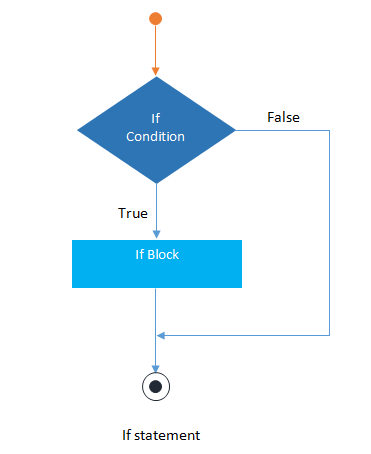
\includegraphics[width=0.2 \textwidth]{ifstatement.png}
		\label{Imagen_if}
	\end{SCfigure}
 
\underline{Instrucción doble condicional}
\\
\textbf{IF-ELSE}
\par{La sentencia if/else extiende la sentencia if especificando una acción if (expresión verdadero/falso) es falso.}
\par{Se puede agregar una cláusula else a un simple condicional para especificar cuales líneas del código a ejecutar si la expresión booleana es falsa. En este caso estamos hablando sobre la estructura if-else, la cual en procesos es expresada de acuerdo con este código.}
\\
If (condición)\\
\{\\
Hacer esto si la condición es verdadera\\
Sentencias if verdaderas\\
\\}\\
else\\
\{\\
Hacer esto si la condición es falsa\\
Sentencias if falsas
\}
\par{Con la sentencia if, un programa se ejecutará el bloque de código verdadero o hará nada. Con la sentencia if/else, el programa ejecutará el bloque del código verdadero o el falso así que siempre algo será ejecutado con una sentencia if/else \cite{iscyp_2017}.}
\begin{itemize}
    \item {Si la expresión es evaluada diferente de cero (verdadera), entonces, el bloque de la sentencia if será ejecutada.}
    \item{Si la expression es evaluada en cero (falsa), entonces, el bloque de la sentencia else será ejecutada.}
\end{itemize}
\begin{SCfigure}[0.8][ht]
	    \centering
		\caption{If-else-ladder, (Obtenida de: {DotNetTricks})}
		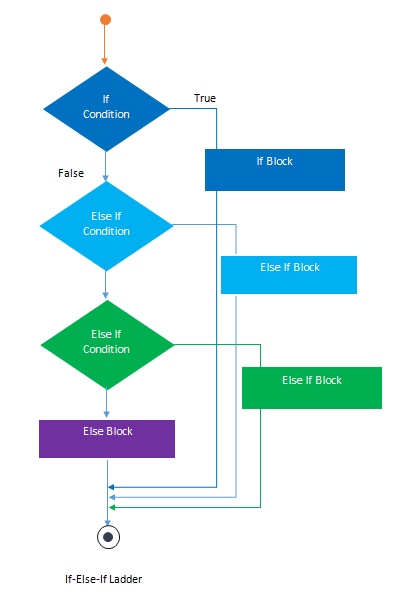
\includegraphics[width=0.2 \textwidth]{if-else-if ladder.png}
		\label{Imagen_If-else}
	\end{SCfigure}
\vspace{0.5 cm}
\underline{Sentencia Multicondicional}\\
\textbf{SWITCH}
\par{Permite una variable para ser comparada con diferentes valores, ejecutando una serie de instrucciones específicas para cada caso. La sentencia switch actúa como un sustituto para un largo if-else-if  Ladder que es usado para probar una lista de casos. Una sentencia switch contiene uno o más casos etiquetados que son probados en contra de la expresión switch. Cuando la expresión coincide con un caso, entonces las sentencias asociadas con ese caso serán ejecutadas.}
\\
La sentencia if-else puede parecer que es innecesario una manera adicional de lidiar con las sentencias condicionales pero basados en ciertos usos, el caso switch fue definido para usar para una sola condición y basado en múltiples casos, el código puede ser ejecutado.
\vspace{0.5 cm}
Switch (expresión) \{ \\
   Caso valor 1: \\
     // Las sentencias son ejecutadas cuando el resultado de la expresión 
     
     coincide con el valor 1
     
     [break;] 
     
     \vspace{0.5 cm}
     
   Caso valor 2: \\
     // Las sentencias son ejecutadas cuando el resultado de la expresión \\ coincide con el valor 2 \vspace{0.5 cm}
     [break;] 
   ... \\
   Caso valor n:\\
     // Las sentencias son ejecutadas cuando el resultado de la expresión \\ coincide con el valor n \vspace{0.5 cm}
     [break;] \\
   default: \\
     // Las sentencias son ejecutadas cuando ninguno de los resultados de la expresión  \\ coincide con el valor de la expresión \vspace{0.5 cm}
     [break;] \\
\} \\
 \begin{SCfigure}[1][ht]
	    \centering
\caption{Switch statement, (Obtenida de: {DotNetTricks})}
		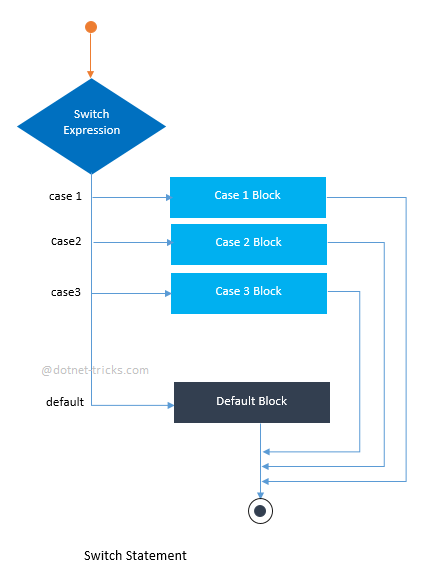
\includegraphics[width=0.5 \textwidth]{switch.png}
		\label{Imagen_Switch}
	\end{SCfigure}
\par{Algunas observaciones sobre esta estructura:
\begin{itemize}
\item Al menos un caso es requerido
\item Si usarás algunos casos, podrías considerar usar if-else en vez de switch-case.
\item La cláusula default es opcional, no estás obligado a ponerla, pero es recomendable.
\item La sentencia break previene procesar de ejecutar las líneas siguientes del caso siguiente.
\end{itemize}
\par{Por ejemplo, si el primer break no ha sido establecido en el ejemplo de arriba, entonces los mensajes “Lunes” y “Martes” serán mostrado. El siguiente ejemplo ayudará a comprender mejor este aspecto.}}\\ \\
\textbf{WHILE}
\par{Es usado cuando queremos repetir la ejecución de sentencias un número indefinido de veces hasta que la condición se cumpla. Es más fácil entender que el bucle for porque no incorpora la inicialización de las variables, sus condiciones para continuar ejecutando y su actualización en la misma línea. Eso sólo indica, como veremos a continuación, la condición que debe cumplirse para que se lleve a cabo una iteración}
   \begin{itemize}
       \item La condición siempre será evaluada antes de cada iteración.
       \item El cuerpo del bucle while se repite hasta que la condición sea verdadera.
       \item El cuerpo del bucle while se ejecuta cero o más veces
   \end{itemize}
\par{Una expresión es evaluada antes de cada paso del loop. Si esta condición evaluada es verdadera, la sentencia será ejecutada. Cuando la condición se evalúa falsa, la ejecución continua con la sentencia después del bucle while}
\begin{SCfigure}[1][ht]
	    \centering
		\caption{Sentencia while, (Obtenida fde: {DotNetTricks})}
		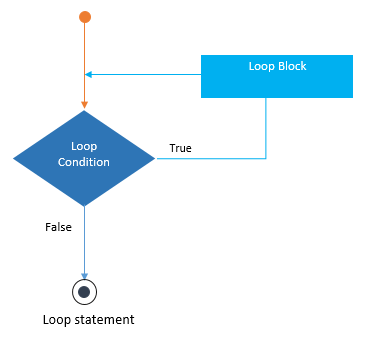
\includegraphics[width=0.2 \textwidth]{cloop.png}
		\label{Imagen_while}
	\end{SCfigure}
	\par{Usualmente, el bucle while es útil cuando no sabes el número exacto de iteraciones.}\\
    \underline{Sentencia de control repetitiva }\\
\textbf{DO-WHILE}\\
\par{Es usado para ejecutar un bloque de instrucciones al menos una vez. El cuerpo del bucle se repite mientras la condición es revisada. Esta condición será evaluada después de cada repetición. Un programa puede ser construido usando una de las sentencias de bucle. Por ejemplo, podemos imprimir números del 1 al 199 usado sólo bucles.}\\ \\
    do\\
    \{ \\
    Instrucción 1 \\
    ... \\
    instrucción n\\
    \} while (condición); \\
\par{Típicamente, para un bucle, es útil cuando sí sabes el número de iteraciones. Normalmente es usado para iterar sobre arreglo y procesos secuenciales.}
    \begin{itemize}
\item El cuerpo del bucle do-while se ejecutará una o más veces.
\item El cuerpo del bucle do-while se repite hasta que la condición es verdadera.
\item La condición siempre será evaluada después de cada iteración.
\end{itemize} \vspace{0.5 cm}
\textbf{For} \vspace{0.5 cm}
\par{Es usado para ejecutar un bloque de instrucciones un número fijo de veces que ya es conocido. Para el bucle for es más conveniente con bucles de conteo. Los bucles están basados en variables de conteo, usualmente conocidos como número de iteraciones. La sentencia puede ser una o un conjunto de ellas (bloque), así que una manera alterna para escribirla puede ser:}\\
    for (CondiciónInicial; ExpresióndePrueba; SentenciaIterativa)\\ 
 \{\\
    Sentencia 1;\\
    Sentencia 2;\\
    // ...\\
   Sentencia N;\\
 \}\\
\par{Cómo funciona:\\
La condición inicial corre una vez, al inicio del bucle
La expresión de prueba es comprobada. (Esto es como la expresión del bucle while). Si es falso, acaba. Si es verdadero,
\begin{itemize}
    \item Corre el cuerpo del bucle
    \item Corre la sentencia iterativa
    \item Regresar al paso de la expresión de prueba y repetir 
\end{itemize}
}
    
  \newpage  





 
    
\newpage

\section{Ejemplos de Modelos Biológicos}
\par{En esta sección le mostramos algunos ejemplos de modelado matemático de otros equipos en iGEM que pueden servir como
referencia para modelar su proyecto. Te invitamos a visitar las wikis de otros equipos para que, como nosotros, te inspires con el
increíble trabajo que han desarrollado otros equipos.}
\subsection{Modelado para decidir qué promotor utilizar}
\par{El equipo Vilnus-Lituania 2021 realizaron modelos matemáticos para elegir pro-motores para modificar la ruta metabólica de su
organismo de una manera óptima.}

\par{Comenzaron usando modelos simples usando la cinética de Michaelis-Menten. Con esto simularon el cambio de producto y
sustrato de su reacción enzimática con respecto al tiempo. Además, construyeron ecuaciones diferenciales para modelar la
concentración de la enzima de interés y su respectivo ARNm.}

\par{Finalmente, modelaron la ruta de síntesis de Naringenina utilizando un sistema de ecuaciones químicas. Este sistema se convirtió a ecuaciones diferenciales. Y, con las suposiciones que hicieron, pudieron simplificar el modelo a unas pocas ecuaciones.}

\begin{SCfigure}[0.65][h]
	    \centering
		\caption{Vía de síntesis de naringenina}
		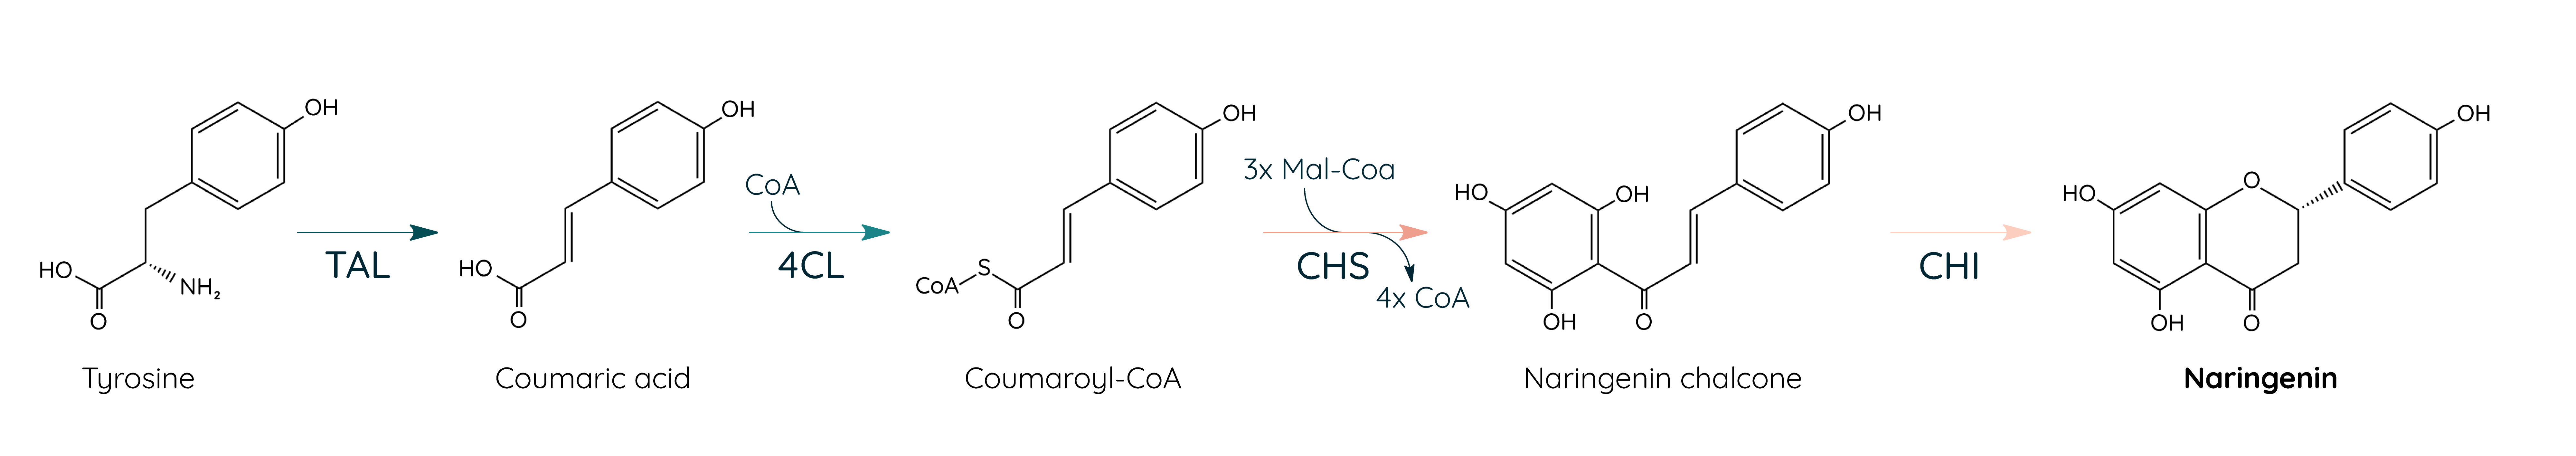
\includegraphics[width=0.65\textwidth]{Vilnus.png}
	\end{SCfigure}

%figura 16

\par{El modelo les ayudó a decidir qué promotor utilizar y pudieron determinar el paso del cuello de botella en la vía de síntesis de la Naringenina.}
    
    \subsection{Modelado del tiempo necesario para producir un componente de interés}
    
\par{Modelar la expresión génica con un sistema de ODEs es una tarea muy común en los proyectos iGEM. Un buen ejemplo de ello
es el trabajo realizado por iGEM Oxford en 2015. Trabajaron en un proyecto que se centró en hacer una alternativa a los antibióticos
para el tratamiento de infecciones urinarias. Para ello, diseñaron Escherichia coli para producir enzimas que pudieran descomponer
las biopelículas bacterianas responsables de la generación de infecciones urinarias. Naturalmente, era necesario saber si sus
bacterias modificadas podrían producir la cantidad necesaria de enzimas. Esta es la parte donde entra el modelado matemático.}

\par{A través de un sistema de EDO, el equipo pudo predecir el tiempo necesario para producir la cantidad deseada de su proteína de interés. Utilizando un sistema de expresión inducido por arabinosa, utilizaron la cinética de Michaelis-Menten para generar su sistema y comparar sus resultados con datos experimentales para ajustarlos. Con estos, pudieron calcular las concentraciones límite de sus productos. Un aspecto destacable de este trabajo es la consideración e investigación de los parámetros de su modelo, lo que le da una gran validez a su modelo.}

    \subsection{Modelado de una reacción de Michaelis-Menten}
\par{Otro ejemplo es el modelo del equipo Queens Canada 2018. Hicieron varios procesos de modelado, pero nos vamos a centrar en
la sección de cinética de Michaelis-Menten que ayuda a analizar la cinética de la enzima.}

\par{En esta parte, hicieron una calculadora que funciona con las entradas de concentración de sustrato, concentración de producto
y concentración de enzima. Esta información se pone en una función que genera la tasa de cambio de concentración. Este
programa se hizo en MATLAB y pusieron el código en su wiki para que otros equipos puedan usar la calculadora en el futuro.}

\begin{SCfigure}[0.65][ht]
	    \centering
		\caption{Los parámetros bien documentados validan el modelo de un equipo y ayudan a los futuros equipos a construir sus propios sistemas \cite{iGEMOxford_2015}}
		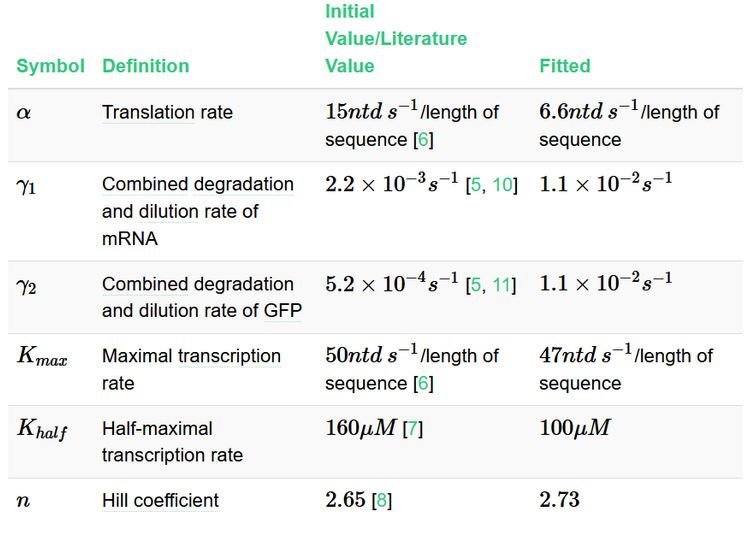
\includegraphics[width=0.65\textwidth]{Tabla parametros.JPG}
	\end{SCfigure}
	\vspace{0.3 cm}


     \subsection{Modelado de la producción, el mecanismo de la entrega y el silenciamiento de
moléculas de miARN}

\par{Para Latinoamérica, la agricultura es una fuente de trabajo e ingreso para millones de personas. Ecuador es país líder en exportación y producción de bananos, esto estaba en riesgo debido a una enfermedad, la marchitez. Por lo que, el equipo de iGEM Ecuador 2021 desarrolló AgroBactory 593, una plataforma bacteriana modular que fabrica biopesticidas utilizando la tecnología de ARNi para combatir enfermedades de las plantas, como la marchitez ocasionada por \textit{Fusarium oxysporum f. sp. cubense} (Foc R4T) en bananos. El medio de entrega de este se planeaba hacer mediante una inyección directa del dsRNA en el tronco y también mediante bacterias de plantas que liberan el dsRNA a través de un sistema de lisis oscilatoria.} 
\par{El dinámico modelo del mismo explicaba la inhibición de los ingredientes activos de Agrobactory con EDOs y dos sistemas de expresión, uno de dsARN y otro del promotor T7 y IPTG para expresión de dsARN.  Este se dividía en tres secciones:}
\begin{enumerate}[1.]
            \item \textbf{Producción de dsRNA} utilizando un promotor constitutivo, las células de Agrobactory producen dsRNA del gen diana.
            \item \textbf{Entrega y liberación de moléculas de dsRNA} a través de una proteína de lisis celular, activada por el mecanismo de detección de quórum que desencadena la lisis celular.
            \item \textbf{Silenciamiento de ARN} del gen Velvet y de cómo las moléculas de interferencia de dsARN y ARN pueden inhibir su expresión génica y controlar la marchitez por \textit{Fusarium}.
\end{enumerate}
\par{Este modelo explica claramente el tipo de modelo que es y qué información se obtendrá gracias al mismo. De igual manera menciona los parámetros utilizados, sus ajustes y se encuentran referenciados. Este ayudó al equipo entender como funcionaba su sistema de expresión y los mecanismos de entrega y silenciamiento, asimismo, emplearon las medidas para entender, desarrollar y mejorar el modelo. }

\par{El modelo es impresionante ya que te permite conocer la producción, el mecanismo del medio de entrega y el silenciamiento del dsRNA de Agrobactory, también utilizaron diagramas que facilitan su comprensión y simulaciones computacionales que comprueban que Agrobactory es funcional. Gracias a esto se pueden hacer predicciones a futuro y son de gran ayuda para otros equipos de iGEM que realizan proyectos similares. }



\newpage

\section{Resumen de programas y modelos}
\par{Las herramientas bioinformáticas pueden ser muy útiles, ya que puedes tener una muy buena idea de lo que estás buscando, como proteínas, sus estructuras en 3D, el enlace entre proteínas, secuencias, cómo va a funcionar tu construcción, modelado de construcciones biológicas, y muchas otras características. Todos estos son esenciales cuando se trabaja en un laboratorio seco porque esta información puede facilitar las cosas cuando se trabaja en el laboratorio húmedo.}

\subsection{Herramientas bioinformáticas}
\par{Hay muchas herramientas de software que pueden facilitar el desarrollo del modelado de sistemas biológicos, modelado de proteínas y simulaciones de interacción molecular. Algunas de estas herramientas también pueden ayudar a analizar el sistema de expresión y ajustar parámetros.}

\begin{table}[]
\begin{tabular}{ | m{3cm} | m{4cm}| m{9.2cm} | } 
\hline
Herramienta &
  Nombre &
  Descripción \\ \hline
\multirow{Software} &
  Cello &
Cello diseña un circuito genético que le proporciona una señal de salida de una serie de datos de entrada, como una secuencia de ADN que codifica la señal de salida deseada a través de especificaciones de sensores, actuadores y restricciones de archivo de usuario. \\ \cline{2-3} 
 &
  Matlab &
  Una plataforma de programación para la resolución de problemas computacionales y matemáticos, como: cálculo matemático, creación de algoritmos, análisis de datos, creación gráfica y modelado de sistemas. SimBiology: un paquete de MatLab que facilita la creación de ecuaciones que describen el comportamiento de un sistema biológico. \\ \hline
\multirow{Modelado de proteínas} &
  I-TASSER &
  Un servidor en línea que puede visualizar las posibles estructuras en la fusión de proteínas, para tener información sobre su función. \\ \cline{2-3} 
 &
  AlphaFold &
  Predice la estructura 3D de una proteína a partir de su amino
secuencias de ácidos. \\ \cline{2-3} 
 &
  Phyre\textasciicircum{}2 &
  Es un motor de reconocimiento de homología/analogía de proteínas, que predice la estructura 3D de una o varias proteínas utilizando secuencias de proteínas o genes.\\ \cline{2-3} 
 &
  PyMOL &
  Es un sistema de visualización molecular para analizar y compartir datos moleculares basado en el software Python.\\ \cline{2-3} 
 &
  UCSF Chimera &
  Permite el acoplamiento molecular entre proteínas y ligandos pequeños de archivos .pdb (Banco de datos de proteínas). \\ \cline{2-3} 
 &
  ArgusLab &
  Es un visor y editor de estructuras biológicas o moléculas orgánicas y permite hacer acoplamiento molecular.\\ \cline{2-3} 
 &
  PyRx &
  Un programa que permite el acoplamiento molecular entre proteínas y pequeños enlaces a través de AutoDock Vina.\\ \cline{2-3} 
 &
  Swiss-Model &
  Un servidor de modelado de homología de estructuras de proteínas totalmente automatizado, accesible a través del servidor web Expasy o el programa DeepView. \\ \cline{2-3} 
 &
  CHARMM-GUI &
  Simplifica y generaliza los protocolos para construir sistemas de simulación complejos y preparar archivos de entrada de simulación para paquetes de simulación ampliamente utilizados. \\ \cline{2-3} 
 &
  HDOCK &
  Es un conjunto altamente integrado de búsqueda de homología, modelado basado en plantillas, predicción de estructuras, acoplamiento macromolecular, información biológica y gestión de trabajos para un acoplamiento proteína-proteína sólido y rápido. \\ \cline{2-3} 
 &
  GLYCAM-Web &
  Predice la estructura 3D de carbohidratos y macromoléculas. \\ \hline
\end{tabular}
\end{table}

\begin{table}[]
\begin{tabular}{|l|l|l|}
\hline
Herramienta &
  Nombre &
  Descripción \\ \hline
\multicolumn{1}{|c|}{\multiro{Parámetros}} &
  C-Score &
  \begin{tabular}[c]{@{}l@{}}Una puntuación de confianza para estimar la calidad de los modelos \\ predichos por I-TASSER. \end{tabular} \\ \cline{2-3} 
\multicolumn{1}{|c|}{} &
  TM-Score &
  Una escala para medir la similitud estructural entre dos estructuras. \\ \cline{2-3} 
\multicolumn{1}{|c|}{} &
  Cluster Density &
  \begin{tabular}[c]{@{}l@{}}Se define como el número de señuelos de estructura en una unidad de \\ espacio en el SPICKER cluster.\end{tabular} \\ \cline{2-3} 
\multicolumn{1}{|c|}{} &
  ERRAT &
  \begin{tabular}[c]{@{}l@{}}Se describe un método para diferenciar entre regiones determinadas \\ correctamente e incorrectamente de estructuras proteicas basándose \\ n la interacción atómica característica.\end{tabular} \\ \cline{2-3} 
\multicolumn{1}{|c|}{} &
  Verify 3D &
  \begin{tabular}[c]{@{}l@{}}Determina la compatibilidad de un modelo atómico (3D) con su\\ propia secuencia de aminoácidos (1D) asignando una clase  \\ estructural basada en su ubicación y entorno (alfa, beta, bucle, \\ polar, no polar, etc.) y comparando los resultados con buenas \\ estructuras.\end{tabular} \\ \cline{2-3} 

\multicolumn{1}{|c|}{} &
  PROVE (z-score) &
  \begin{tabular}[c]{@{}l@{}}Calcula los volúmenes de átomos en macromoléculas mediante un \\ algoritmo que trata a los átomos como esferas duras y calcula una \\ desviación de puntuación Z estadística para el modelo a partir de \\ estructuras depositadas en PDB altamente resueltas \\ y refinadas.\end{tabular} \\ \cline{2-3} 
\multicolumn{1}{|c|}{} &
  PROCHECK &
  \begin{tabular}[c]{@{}l@{}}Comprueba la calidad estereoquímica de la estructura de una proteína \\ mediante el análisis de la geometría residuo por residuo y la \\ geometría de la estructura general.\end{tabular} \\ \hline
\multirow{\begin{tabular}[c]{@{}l@{}}Molecular\\ Interaction\\ Simulation\end{tabular}} &
  GROMACS &
  \begin{tabular}[c]{@{}l@{}}Un programa multiplataforma de código abierto para realizar\\ simulaciones de dinámica molecular y minimización de energía de\\ sistemas con cientos de millones de partículas.\end{tabular} \\ \cline{2-3} 
 &
  AutoDocs &
  \begin{tabular}[c]{@{}l@{}}Un software de simulación de modelos moleculares diseñado para\\ predecir la unión entre moléculas pequeñas y receptores con \\ estructuras tridimensionales conocidas.\end{tabular} \\ \cline{2-3} 
 &
  ClusPro &
  \begin{tabular}[c]{@{}l@{}}Un servidor utilizado para el análisis estructural de un \\ acoplamiento proteína-proteína y los resultados obtenidos \\ pueden permitir la identificación de las mejores conformaciones \\ de acoplamiento.\end{tabular} \\ \cline{2-3} 
 &
  PIPER &
  \begin{tabular}[c]{@{}l@{}}Un programa de ajuste basado en el método de correlación Fast\\ Fourier Transform (FFT) y se utiliza en el paso de ajuste de \\ cuerpo rígido.\end{tabular} \\ \cline{2-3} 
 &
  PatchDock &
  \begin{tabular}[c]{@{}l@{}}Utiliza una técnica similar a un rompecabezas. Dadas dos\\ moléculas, sus superficies se dividen en partes según la forma\\ de la superficie. Estas piezas corresponden a patrones\\ visualmente distinguibles. Una vez que se identifican los \\ fragmentos, se pueden superponer utilizando algoritmos de\\ formas coincidentes.\end{tabular} \\ \cline{2-3} 
 &
  FireDock &
  \begin{tabular}[c]{@{}l@{}}Un software para el análisis y puntuación de soluciones de\\ acoplamiento proteína-proteína.\end{tabular} \\ \cline{2-3} 
 &
  PyDock &
  \begin{tabular}[c]{@{}l@{}}Un servidor web para la predicción de acoplamiento de cuerpo\\ rígido de estructuras complejas proteína-proteína canta una\\ nueva versión del algoritmo de puntuación pyDock.\end{tabular} \\ \hline
\end{tabular}
\end{table}

\newpage

\subsection{Herramientas informáticas para la modelización}
\par{Para construir un modelo matemático, necesitamos seleccionar la estructura de ecuaciones diferenciales, que se transformará
en un sistema con muchas incógnitas empleando métodos numéricos. Para hacer eso, usamos la programación:}

\begin{table}[h]
\begin{tabular}{| m{3cm} | m{9cm}|}
\hline
\multicolumn{1}{|c|}{\textbf{Lenguajes de programación}}                                                                                                           \\ \hline
\multicolumn{1}{|l|}{C} & Los programas grandes se dividen en programas pequeños llamados funciones que se centran en funciones y procesos que operan con datos. \\ \hline
\multicolumn{1}{|l|}{C\#} &
  Un lenguaje de programación multiparadigma con sólidas disciplinas de programación en escritura, imperativas, declarativas, funcional y orientado a objetos. \\ \hline
\multicolumn{1}{|l|}{C++}    & Una extensión del lenguaje C, pero de nivel medio y orientado a objetos.                                                  \\ \hline
\multicolumn{1}{|l|}{Python} & Un lenguaje interpretado, orientado a objetos y construido sobre una semántica flexible y robusta.                                    \\ \hline
\multicolumn{1}{|l|}{Ruby}   & Un lenguaje de secuencias de comandos orientado a objetos de código abierto que se puede usar de forma independiente o como parte del marco web de Ruby on Rails. Un lenguaje de secuencias de comandos.   \\ \hline
\multicolumn{1}{|l|}{PHP}    & Código abierto diseñado para crear páginas web dinámicas que funcionan de manera efectiva con bases de datos.                    \\ \hline
\multicolumn{1}{|l|}{Java}   & Un lenguaje de programación orientado al usuario de alto nivel, ideal para el desarrollo basado en la web.                                              \\ \hline
\multicolumn{1}{|l|}{JavaScript} &
  Un lenguaje de programación que se ejecuta dentro de un navegador de cliente y procesa comandos en una computadora en lugar de un servidor. \\ \hline
\end{tabular}
\end{table}


\subsection{Modelos a utilizar}
\par{Los modelos matemáticos se pueden clasificar en función de diversas características. Hay una gran cantidad de clasificaciones diferentes para los modelos matemáticos. No obstante, aquí resumimos algunos de ellos, su finalidad y un ejemplo de un equipo iGEM que los ha utilizado.} 

\begin{table}[h]

\begin{tabular}{ | m{3cm} | m{7cm}| m{6.2cm} | } 
\hline
\textbf{Tipo de Modelo} & {\color[HTML]{000000} \textbf{Descripción Breve}}                                                                                                    & \multicolumn{1}{c|}{\textbf{Ejemplo}}                                  \\ \hline
Determinístico                                 & Cada valor de parámetro se puede representar como un número concreto.                                                                                        & El TuDelft iGEM Team 2021 utiliza un modelo determinista para representar la red biomolecular de AptaVita (su proyecto)\\ \hline
Estocástico                                    & Cada parámetro se puede representar como un conjunto de valores aleatorios definidos con distribuciones de probabilidad.                                                  & Thessaly 2021 iGEM Team utiliza ambos (modelos deterministas y estocásticos) para simular su proyecto in silico.             \\ \hline
Método Monte Carlo                            & Esta es una técnica matemática utilizada para los posibles resultados de un evento incierto.                                                             &   Evaluar el impacto del riesgo en el precio de las acciones. %https://www.ibm.com/es-es/cloud/learn/monte-carlo-simulation                                                                                                                      
\\ \hline
Optimización                                  & Este tipo de modelo se utiliza para encontrar los parámetros óptimos del objeto de estudio.                                                                     & Encontrar la masa más pequeña posible de un cohete lanzado desde algún lugar para llegar a una parte exacta del espacio.            \\ \hline
Caótico                                       & Este modelo utiliza ideas de la teoría del caos para abordar problemas comunes mientras se trabaja en equipo. Generalmente se utiliza como metodología de programación. & Cómo la contaminación de la Ciudad de México influye en el turismo de la ciudad.                                                            \\ \hline
Complejo                                       & Los elementos del sistema y el sistema mismo interactúan con los elementos del mundo circundante, y estas interacciones pueden cambiar con el tiempo. & Modelización del tráfico de una ciudad.                                                                                \\ \hline
    
\end{tabular}
\end{table}

\newpage 
\subsection{Sentencias de control}
\par{Los tres tipos de condicionales (simple, doble y múltiple) permiten que el programa ejecute ciertas líneas de código cuando se cumple una condición, siempre que se cumpla una condición. En resumen, las sentencias de control son las siguientes:}

\begin{center}
\begin{tabular}{ | m{3cm} | m{4cm}| m{9.2cm} | } 
\hline
Sentencia & Tipo de condicional & Función \\\hline
If & Simple & Ejecutar líneas de código si se cumple una condición. \\\hline
Else & Simple & Cláusula agregada a un condicional simple para ejecutar líneas de código si no se cumple una condición. \\\hline
Switch & Doble & Compara una variable con posibles valores y ejecuta el que se cumple. \\\hline
While & Doble & Repite una declaración siempre que se cumpla una condición. \\\hline
Do-While & Repetitivo & Ejecuta una declaración al menos una vez y la repite siempre que se cumpla una condición. \\\hline
For & Repetitivo & Ejecuta código un número fijo de veces.\\\hline
\end{tabular}
\end{center}


\newpage 

\bibliographystyle{apalike}
\bibliography{ref}

\end{document}